% ============= Settings for the Work =============

%***************************************************************************************

% Place your data here!!!

\def\workTitle{Praxissemesterbericht}
\def\subTitle{Fullstack SAP Entwicklung}
\def\specialization{<Name of Masterclass>}
\def\typeOfWork{Paxissemesterbericht}
\def\courseOfStudy{Bachelor-Studiengang Informatik}
\def\universityName{Hochschule Mannheim}
\def\faculty{Fakultät für Informatik}
\def\studentFirstName{Luc}
\def\studentLastName{Dreibholz}
\def\studentId{2210544}
\def\advisorPreTitle{}
\def\advisoFirstName{Oliver}
\def\advisorLastName{Schmitt}
\def\advisorPosTitle{}
\def\assessorPreTitle{}
\def\assessorFirstName{}
\def\assessorLastName{}
\def\assessorPosTitle{}
\def\place{Mannheim}
\def\dateDay{11}
\def\dateMonth{06}
\def\dateYear{2024}

%***************************************************************************************

\newif\ifUseOneSide                         % <== DONT TOUCH THIS!!!
\newif\ifUseGermanVersion				    % <== DONT TOUCH THIS!!!
\newif\ifUseMasterInteractiveTechnologies 	% <== CAN'T TOUCH THIS!!! (da da dada)
\newif\ifUseMasterDigitalDesign	            % <== DONT TOUCH THIS!!!
\newif\ifUseMasterDigitalMediaProduction	% <== DONT TOUCH THIS!!!
\newif\ifUseMasterDigitalHealthCare			% <== DONT TOUCH THIS!!!
\newif\ifUseBachelorMediaTechnologies       % <== DONT TOUCH THIS!!!
\newif\ifUseBachelorSmartEngineering        % <== DONT TOUCH THIS!!!
\newif\ifUseBachelorCreativeComputing       % <== DONT TOUCH THIS!!!

%To switch between one or two side layout
\UseOneSidetrue                             % Using the one side layout
%\UseOneSidefalse                            % Using the two side layout
% *** ATTENTION: When using double page layout, you need to print the Title Page as a single Page!!! ***

%***************************************************************************************

% To switch the version please use the comment "%" option :-). After a language change, you have to rebuild the whole project (in Overleaf --> recompile from scratch) 
\UseGermanVersiontrue					    % German version
% \UseGermanVersionfalse					    % English version

%***************************************************************************************

% To switch between the study programs use the comment option :-) 
% !!!ATTENTION: Only one has to be activated!!!

%\UseBachelorMediaTechnologiestrue		   % Bachelor Media Technology
%\UseBachelorSmartEngineeringtrue		    % Bachelor Smart Engineering
\UseBachelorCreativeComputingtrue		    % Bachelor Creative Computing
%\UseMasterInteractiveTechnologiestrue		% Master Interactive Technologies
%\UseMasterDigitalDesigntrue		        % Master Digital Design
%\UseMasterDigitalMediaProductiontrue		% Master Digital Media Production
%\UseMasterDigitalHealthCaretrue			% Master Digital Health Care

%***************************************************************************************
%Dokumentklasse without end dot ;-)
%\documentclass[a4paper,twoside,11pt, numbers=noenddot]{scrreprt
%\PassOptionsToPackage[english,ngerman]{babel}
\ifUseOneSide
    \documentclass[a4paper,oneside,11pt, numbers=noenddot]{scrreprt}%{book}{report}
\else
    \documentclass[a4paper,twoside,11pt, numbers=noenddot]{scrreprt}%{book}{report}
\fi
\usepackage[ngerman, english]{babel}
\usepackage[left= 3.5cm,right = 3cm, bottom = 3.5 cm, top = 3 cm]{geometry}
\usepackage[onehalfspacing]{setspace}

% Standard Packages
\usepackage[utf8]{inputenc}

% ============= Packages =============
\usepackage{acronym}

% Document information
\usepackage[
	pdftitle={\workTitle},
	pdfsubject={},
	pdfauthor={\studentFirstName \studentLastName},
	pdfkeywords={}
	pdftex=true, 
	colorlinks=true,
 	breaklinks=true,
	citecolor=black,
	linkcolor=black,	
	menucolor=black,	
	urlcolor=black
]{hyperref}

\hypersetup{
    %bookmarks=true,         % show bookmarks bar?
    unicode=true,          % non-Latin characters in Acrobat’s bookmarks
    pdftoolbar=true,        % show Acrobat’s toolbar?    pdfmenubar=true,        % show Acrobat’s menu?
    pdffitwindow=false,     % window fit to page when opened
    pdfstartview={FitH},    % fits the width of the page to the window
    pdftitle={My title},    % title
    pdfauthor={Author},     % author
    pdfsubject={Subject},   % subject of the document
    pdfcreator={Creator},   % creator of the document
    pdfproducer={Producer}, % producer of the document
    pdfkeywords={keyword1} {key2} {key3}, % list of keywords
    pdfnewwindow=true,      % links in new window
    colorlinks=false,       % false: boxed links; true: colored links
    linkcolor=black,          % color of internal links (change box color with linkbordercolor)
    citecolor=black,        % color of links to bibliography
    filecolor=black,      % color of file links
    urlcolor=black           % color of external links
}

\usepackage{csquotes}

\usepackage[T1]{fontenc}
\usepackage{graphicx, subcaption}
\usepackage{fancyhdr}
\usepackage{lmodern}
\usepackage{color}
\usepackage{colortbl}
\usepackage{transparent}

%\usepackage[style=numeric, backend=biber]{biblatex}

%\usepackage[backend=biber, style=apa, citestyle=authoryear, sorting=nyt]{biblatex}
\usepackage[backend=biber, style=ieee, citestyle=numeric, sorting=nyt]{biblatex}
%\usepackage[backend=biber, style=ieee, sorting=nyt]{biblatex}
% Usable sorting styles are:
% nty = Sort by name, title, year.
% nyt = Sort by name, year, title.
% nyvt = Sort by name, year, volume, title.
% anyt = Sort by alphabetic label, name, year, title.
% anyvt = Sort by alphabetic label, name, year, volume, title.
% ynt = Sort by year, name, title.
% ydnt = Sort by year (descending), name, title.
% none = Do not sort at all. All entries are processed in citation order.
% debug = Sort by entry key. This is intended for debugging only.

\addbibresource{biblatex.bib}

% Additional letters from the American Mathematical Society
\usepackage{amsfonts}
\usepackage{mathtools}

\usepackage[export]{adjustbox}

% Block Diagram Drawing Package
% ---tikz
\usepackage{tikz}
\usetikzlibrary{positioning}
\usepackage{pgfplots}
\pgfplotsset{compat=1.10}
\usepackage{textcomp}

%Package for using the [H] option on graphics to force them into place
\usepackage{float}

%iPython packages:
%\usepackage{graphicx} % Used to insert images
\usepackage{adjustbox} % Used to constrain images to a maximum size 
\usepackage{color} % Allow colors to be defined
\usepackage{enumerate} % Needed for markdown enumerations to work
\usepackage{geometry} % Used to adjust the document margins
\usepackage{amsmath} % Equations
\usepackage{enumitem,amssymb} % Equations
\newlist{todolist}{itemize}{2} % for declaration
\setlist[todolist]{label=$\square$}
%\usepackage[mathletters]{ucs} % Extended unicode (utf-8) support
% \usepackage[utf8x]{inputenc} % Allow utf-8 characters in the tex document
\usepackage{fancyvrb} % verbatim replacement that allows latex
\usepackage{grffile} % extends the file name processing of package graphics 
                         % to support a larger range 
    % The hyperref package gives us a pdf with properly built
    % internal navigation ('pdf bookmarks' for the table of contents,
    % internal cross-reference links, web links for URLs, etc.)
\usepackage{hyperref}
\usepackage{longtable} % longtable support required by pandoc >1.10

% embedding of audio/video files etc.
% \usepackage{attachfile}
% \usepackage{movie15}
% \usepackage{media9}
% \usepackage{menukeys}

\usepackage[labelfont=it, labelsep=period, format=plain,justification=raggedright, singlelinecheck=false]{caption}
\captionsetup[figure]{justification=centering}
\definecolor{light-gray}{gray}{0.85}

% Switch between German and English based on the Settingx.tex. file
\usepackage{ifthen}

% =============== Block Diagram Drawing Config
\usetikzlibrary{shapes,arrows}

% Definition of blocks:
\tikzset{%
  block/.style    = {draw, thick, rectangle, minimum height = 3em,
    minimum width = 3em},
  sum/.style      = {draw, circle, node distance = 2cm}, % Adder
  input/.style    = {coordinate}, % Input
  output/.style   = {coordinate}, % Output
  mult/.style	  = {draw, isosceles triangle, minimum height=1cm, minimum width =1cm}
}
%mult/.style	  = {isosceles triangle, sharp corners, anchor=center, xshift=-4mm, minimum height=1.5cm, minimum width =0.05cm}
%isosceles triangle, fill=gray!25, minimum width=1.5cm

% Defining string as labels of certain blocks.
\newcommand{\suma}{\Large$+$}
\newcommand{\inte}{$\displaystyle \int$}
\newcommand{\derv}{\huge$\frac{d}{dt}$}
\newcommand{\conv}{\huge$\ast$}

% ============================================

% -- Settings für Code abbildungen
\usepackage{listings,lstautogobble}

\definecolor{lightgray}{rgb}{.9,.9,.9}
\definecolor{darkgray}{rgb}{.4,.4,.4}
\definecolor{purple}{rgb}{0.65, 0.12, 0.82}

\lstdefinelanguage{JavaScript}{
  keywords={typeof, new, true, false, catch, function, return, null, catch, switch, var, if, in, while, do, else, case, break, interface, log, let, const, class, import, from, export, extends, public, private},
  keywordstyle=\color{blue}\bfseries,
  ndkeywords={export, boolean, throw, implements, this, number, string},
  ndkeywordstyle=\color{darkgray}\bfseries,
  identifierstyle=\color{black},
  sensitive=false,
  comment=[l]{//},
  morecomment=[s]{/*}{*/},
  commentstyle=\color{purple}\ttfamily,
  stringstyle=\color{red}\ttfamily,
  morestring=[b]',
  morestring=[b]"
}

\lstset{
   language=JavaScript,
   backgroundcolor=\color{lightgray},
   extendedchars=true,
   basicstyle=\footnotesize\selectfont,
   showstringspaces=false,
   showspaces=false,
   frame=leftline,
   numbers=left,
   numberstyle=\footnotesize,
   numbersep=9pt,
   tabsize=2,
   breaklines=true,
   showtabs=false,
   captionpos=b,
   autogobble=true
}

% Setze arial font
\usepackage[scaled]{helvet}
\renewcommand*{\familydefault}{\sfdefault}

% FH-green blue
\definecolor{FH}{rgb}{0.10, 0.57, 0.68}
% FH-green blue 2
\definecolor{FH2}{rgb}{0.0392, 0.666, 0.549}
% TitlePage Title color
\definecolor{TitleHeader}{HTML}{44B94B}

% No indention afer a paragraph
\setlength{\parindent}{0cm}

% Paragraph
\setlength{\parskip}{0.3cm}

% ============= Header and Footer =============

\renewcommand{\chaptermark}[1]{\markboth{\thechapter~ #1}{}}

\ifUseOneSide
\fancypagestyle{icmt}{%
  \fancyhf{}% Clear header and footer
  \fancyhead[L]{\leftmark}
  \fancyfoot[R]{\thepage}% Custom footer
  \renewcommand{\headrulewidth}{0.4pt}% Line at the header visible
  \renewcommand{\footrulewidth}{0.0pt}% Line at the footer visible
}
% Redefine the plain page style
\fancypagestyle{plain}{%
  \fancyhf{}%
  \fancyfoot[R]{\thepage}%
  \renewcommand{\headrulewidth}{0.0pt}% Line at the header invisible
  \renewcommand{\footrulewidth}{0.0pt}% Line at the footer visible
}
\else
\fancypagestyle{icmt}{%
  \fancyhf{}% Clear header and footer
  \fancyhead[L]{\leftmark}
  \fancyfoot[RO,LE]{\thepage}% Custom footer
  \renewcommand{\headrulewidth}{0.4pt}% Line at the header visible
  \renewcommand{\footrulewidth}{0.0pt}% Line at the footer visible
}
% Redefine the plain page style
\fancypagestyle{plain}{%
  \fancyhf{}%
  \fancyfoot[RO,LE]{\thepage}%
  \renewcommand{\headrulewidth}{0.0pt}% Line at the header invisible
  \renewcommand{\footrulewidth}{0.0pt}% Line at the footer visible
  }
\fi

% ============= Package Settings & Others ============= 


% Special Spellings
\hyphenation{De-zi-mal-tren-nung St-rei-fen-licht-scan-nern}

% Roman itemization \RM{<Number>}
\newcommand{\RM}[1]{\MakeUppercase{\romannumeral #1}}


% ============= Dokumentbeginn =============

\begin{document}
\selectlanguage{ngerman}

% Select the right main page ;-)

% setup page dimensions for titlepage
\newgeometry{left=2.4cm,right=2.4cm,bottom=2.5cm,top=2cm}


% first titlepage
\pagestyle{empty}

\vspace*{-2cm}
\begin{figure}[H]
	\setlength{\fboxrule}{0pt}
	\fbox{\begin{minipage}[t!]{150pt}
		
\includegraphics[width=150pt]{TemplateElements/HSMALogo.png}
	\end{minipage}}
	\hfill
	\fbox{\begin{minipage}[t!]{150pt}
		
\includegraphics[width=150pt]{TemplateElements/sovantaLogo.jpg}
	  \end{minipage}}
\end{figure}


\begin{center}

\vspace{1cm}

\begin{minipage}[t][5cm][s]{\textwidth}%
\centering
\Huge{{\color{TitleHeader}{\fontsize{24}{30} \selectfont \workTitle\\}}}
\vspace{0.5cm}
\LARGE{{\color{TitleHeader}{\fontsize{16}{24} \selectfont \subTitle\\}}}
\end{minipage}

Vorgelegt von:\\ 
\fontsize{15pt}{15pt}\selectfont
\textbf{\studentFirstName\ \studentLastName} \\
\fontsize{11pt}{15pt}\selectfont
Matr.Nr.: \studentId \\
\courseOfStudy
  
\vspace{1.3cm}
    	\fontsize{11pt}{15pt}\selectfont \universityName\\ 
	\faculty \\

\vspace{1.3cm}
    	\fontsize{11pt}{15pt}\selectfont Unternehmen: \\
		\textbf{sovanta AG}\\ 
		Mittermaierstraße 31 \\
		69115 Heidelberg

\vspace{1cm}

\begin{tabular}{lll}
	Betreuer/in: & \advisorPreTitle\ \advisoFirstName\ \advisorLastName \advisorPosTitle\\
\end{tabular}

\vspace{1cm}

\begin{tabular}{lll}
	\fontsize{11pt}{15pt}\selectfont Praktikumszeitraum: & 01.03.2024 - 26.07.2024\\
	Fertigstellung: & \dateDay.\dateMonth.\dateYear
\end{tabular}


\end{center}

\restoregeometry


% \part No numbering in the table of contend
\makeatletter
\let\partbackup\l@part
\renewcommand*\l@part[2]{\partbackup{#1}{}}

% Restart of the page numbering, Numbers [arabic], Roman numbers [roman,Roman], letters [alph,Alph]
\pagenumbering{Roman}

\pagestyle{plain}
\chapter*{Sichtvermerk der Firma:}
\label{ch:erklaerung}

\begin{flushleft}
	Firmenstempel und Unterschrift der betreuenden Person(en)
\end{flushleft}
\vspace{1cm}
\begin{flushleft}
	Datum:	\hrulefill\enspace Unterschrift: \hrulefill
\end{flushleft}
\begin{flushleft}
	Datum:	\hrulefill\enspace Unterschrift: \hrulefill
\end{flushleft}

	

\newpage

% Table of Contend
\tableofcontents

\newpage
% Restart of the page numbering, Numbers [arabic], Roman numbers [roman,Roman], letters [alph,Alph]
\pagenumbering{arabic}

% Activate page style for the whole document
\pagestyle{icmt}
\newpage

% /*================================
% =            CONTENTS            =
% ================================*/

% \chapter{Firmenumfeld und Zielsetzung der Arbeit}
\label{ch:introduction}

\section{Firmenumfeld}
Die sovanta AG ist ein in Heidelberg ansässiges Unternehmen, das sich auf die Entwicklung von Softwarelösungen für Unternehmen spezialisiert hat.
Besonders im Bereich der SAP-Anwendungen ist sovanta darauf fokussiert, komplexe Geschäftsprozesse durch benutzerfreundliche und effiziente Lösungen zu verbessern.
Das Unternehmen arbeitet eng mit verschiedenen Kunden aus unterschiedlichen Branchen zusammen, um maßgeschneiderte Software zu entwickeln, die genau auf deren Bedürfnisse abgestimmt ist.

Das Arbeitsumfeld bei sovanta zeichnet sich durch eine offene und teamorientierte Atmosphäre aus.
In den Projektteams wird oft mit agilen Methoden wie Scrum gearbeitet, was eine flexible und dynamische Arbeitsweise ermöglicht.
Der regelmäßige Austausch innerhalb der Teams und mit den Kunden spielt dabei eine wichtige Rolle, um schnell auf neue Anforderungen reagieren und eine hohe Qualität sicherstellen zu können.
Die Kombination aus technischer Expertise und einer starken Fokussierung auf die Bedürfnisse der Nutzer ist ein wesentlicher Bestandteil der Firmenphilosophie von sovanta.

\section{Zielsetzung der Arbeit}
Während meines Praktikums war ich Teil eines agilen Scrum-Teams, das eine SAP-Anwendung für ein großes Unternehmen entwickelte.
Ich arbeitete an Features sowohl im Frontend als auch im Backend.

Zusätzlich habe ich Bugs gefixt, um die Anwendung stabiler zu machen.
Ein weiterer wichtiger Teil meiner Arbeit war das Schreiben von Tests, um die Qualität des Codes sicherzustellen.

Meine Aufgabe bestand darin, das Projekt voranzutreiben, indem ich neue Funktionen entwickelte und die bestehende Code-Qualität verbesserte.
\chapter{Wochenberichte}
\label{ch:wochenberichte}

\section{Einarbeitung in das \acs{sapui5} Frontend Framework}
In meiner ersten Praktikumswoche begann mit einem kurzen technischen Onboarding, indem mir mein Equipment bereitgestellt und alle sovanta-Accounts eingerichtet wurden. Danach habe ich mich intensiv mit dem \acs{sapui5}-Framework auseinandergesetzt. Ziel war es, eine umfassende Einführung in die Grundlagen dieses Frameworks zu erhalten. Dabei lag der Fokus auf dem Verständnis von \acs{sapui5}-spezifischen Konzepten wie Data Binding, Fragments, Views und Routing. \\\\
Die Einarbeitung begann ich mit einer Analyse der Dokumentation und Online-Ressourcen, um ein solides Fundament zu legen. Dabei kamen insbesondere Fragen zum effektiven Einsatz von Data Binding und zur korrekten Implementierung von Fragments auf. \\\\
Die Herausforderung bestand darin, die theoretischen Kenntnisse in der praktischen Anwendung zu vertiefen. Durch aktives Experimentieren und Umsetzen kleiner Beispiele gelang es mir, die Zusammenhänge besser zu verstehen. Schwierigkeiten traten vor allem bei der korrekten Integration von Data Binding-Funktionalitäten auf, wobei ich auf Online-Foren und Tutorials zurückgriff, um Lösungsansätze zu finden. \\\\

\section{Vertiefung der \acs{sapui5} Kenntnisse und \acs{cap} Backend Framework}
Die zweite Woche meines Praktikums stand ganz im Zeichen der Vertiefung meines Verständnisses für das \acs{sapui5}-Frontend-Framework und dem dazugehörigen \acs{cap} Backend-Framework. \\\\
Aufgrund von Problemen mit dem Zugang zu der Codebase des Projektes, dem ich zugeteilt wurde, verzögerte sich die Einarbeitung in die Codebase, an der ich die nächsten Monate arbeiten werde. Diese Zeit nutzte ich jedoch effektiv, indem ich mich eigenständig den fortgeschrittenen Konzepten von \acs{sapui5} und der den Grundlagen von \acs{cap} widmete. Hierbei fing ich an die Dokumentation für das \acs{cap} Framework zu lesen und erste kleine Projekte aufzusetzen. \\\\
Die größte Herausforderung dieser Woche war es, die erworbenen Kenntnisse in der Praxis anzuwenden und eine Verbindung zwischen einer eigenen \acs{sapui5}-Anwendung und dem \acs{cap} Backend herzustellen und vor allem das Konzept des OData Datenmodells zu verstehen und zu implementieren, welches für SAP-Anwendungen essenziell ist. \\\\
Durch kontinuierliche Experimente und die Analyse von Beispielcode gelang es mir jedoch, ein tieferes Verständnis für dieses Datenmodell zu gewinnen und dieses Verständnis in einer ersten Anwendung mit einem \acs{sapui5} Frontend und \acs{cap} Backend umzusetzen. \\\\

\section{Einarbeitung in die Project-Codebase und erste eigene Tickets}
In der dritten Woche konnte ich endlich auf die Codebase des Projekts zugreifen, was mir die Einarbeitung in das laufende Projekt ermöglichte. Nachdem ich mich mit der Codebase etwas vertraut gemacht hatte, konnte ich mich auch direkt aktiv in das laufende Projekt einbringen, indem ich meine ersten eigenen Tickets bearbeitete. Diese Tickets beinhalteten die Implementierung verschiedener Features und Anpassungen, um die Funktionalität und Benutzerfreundlichkeit der Anwendung zu verbessern. \\\\
Die Hauptaufgabe diese Woche bestand darin, einen neuen Filter und eine neue Spalte, für bestehende Werte aus der Datenbank, zur Tabelle aller Kaufprojekte auf der Übersichtsseite hinzuzufügen. Zusätzlich zu dieser größeren Aufgabe bearbeitete ich auch kleinere Tickets, wie das Ändern von Dropdown-Optionen, die Anpassung von Abkürzungen in der gesamten Anwendung und das automatische Befüllen des "Währung"-Felds beim Erstellen eines bestimmten neuen Kaufprojektes. \\\\
Die größte Herausforderung bestand darin, die komplexe Codebase und Architektur eines schon so großen Projektes zu verstehen und dann an den richtigen Stellen Änderungen zu machen, um die Ergebnisse zu erzielen, die gefordert waren. Diese Heraufforderung konnte ich durch viel ausprobieren und befragen meines Betreuers, zumindest teilweise, bewältigen. \\\\

\section{Erstes Sprint Review und weitere Bearbeitung von Tickets}
Diese Woche lief ähnlich wie letzte Woche und ich arbeitete weiter an eigenen Tickets. Dazu kam dann allerdings auch, dass in dieser Woche das Sprint Review anstand, in dem ich dann die Ergebnisse, die ich in diesem Sprint erreicht habe, vor dem Kunden präsentieren sollte. \\\\
Für das Sprint Review habe ich mich vorher mit meinem Betreuer zusammengesetzt und er hat mir erklärt, wie das Review abläuft und wie er sich darauf vorbereitet. Anhand dieser Informationen habe ich mir dann einen Plan gemacht, was ich wie vorstellen möchte. Dafür habe ich dann auf dem Development System Beispiel Kaufprojekte angelegt, um daran die Änderungen besser vorstellen zu können und einen reibungslosen Ablauf zu garantieren. \\\\
Nach dem Review folgte dann das Sprint Planning, in dem mir dann eine neue, etwas größere, Aufgabe zugeteilt wurde. Die Aufgabe besteht darin, in der ganzen Anwendung die Länder und Ländercodes in eine, von dem Kunden vorgegebene, einheitliche Reihenfolge zu bringen. Dafür musste ich zuerst eine Liste mit allen Vorkommnissen von Ländern in der Anmeldung machen und deren Ursprung im Code herausfinden. \\\\
Diese Aufgabe zu lösen, stellte sich als größere Herausforderung heraus als eigentlich gedacht, da die Ländercodes an viele Stellen auch als zusammengesetzter String in den Datenbanktabellen der Kaufprojekte stehen und so diese Werte, bei bestehenden Projekten, nicht so einfach neu sortiert werden können. Für dieses Problem konnte ich diese Woche allerdings noch keine Lösung finden. \\\\

\section{Reihenfolge der Länder in der ganzen Anwendung ändern}
Diese Woche widmete ich mich vollkommen der Aufgabe eine Lösung für die neue Sortierung aller Ländervorkommnisse in der Anwendung zu finden. \\\\
Das größte Problem war hierbei, dass Kaufprojekte zum einen so genannte countryCodes beinhalteten, welche eine Zugehörigkeit zu diesen Ländern aussagt. Aber auch ein countryLabel, welches ein im Backend berechneter String ist, welcher die countryCodes mit einem Trennzeichen miteinander verknüpft und in der Datenbank speichert. Da es keine Option war, in der Datenbank alle countryLabel, mit der neuen Reihenfolge zu aktualisieren, musste ich hier im Backend die Rückgabe der Projekte modifizieren. Bevor diese dann an das Frontend gesendet wurden, mussten diese, getrennt, neu sortiert und dann wieder mit dem richtigen Trennzeichen zusammenfügt werden. \\\\
Ein weiteres Problem war, dass nicht nur Projekte eine Zughörigkeit zu einem oder mehreren Ländern haben, sondern es viele verschiedene Entitäten gibt, welche einen Ländercode gespeichert haben. Dieser Code war allerdings in vielen Fällen unter einem anderen Namen in den Entitäten zu finden. Das machte es schwierig, eine einzelne Funktion zum Sortieren all dieser Sonderfälle zu erstellen. Dafür musste ich die Sonderfälle separat abfragen und je nach Entität ein anderes Attribut zum Sortieren verwenden. \\\\

\section{Fertigstellung der Länderreihenfolge und eine neue Aufgabe}
Am Anfang dieser Woche habe ich mich Hauptsächlich damit beschäftigt, die letzten Fehler, die beim Testen des Features, mit dem ich mich die letzte Woche beschäftigt habe, aufgekommen sind, zu beheben. \\\\
Das größte Problem war, dass das Sortieren in manchen Fällen nicht so funktioniert hat wie es sollte. Das lag daran, dass wir uns dazu entschieden haben, sogenannte Streams, welche mehreren Ländern zugehörig waren, anhand des ersten Landes in der Liste der Länder zu sortieren. Das hatte zur Folge, dass, wenn es mehrere Streams in einem Kaufprojekt gibt, welche mit demselben Land anfingen und eine unterschiedliche Anzahl an Ländern hatten, die Sortierung nicht mehr richtig funktioniert hat. Um dieses Problem zu beheben, musste die Sortierfunktion angepasst werden. Hier entschied ich mich, zusammen mit meinem Betreuer, dazu die Länder, die mit demselben Land beginnen, anhand der Länge der Länderliste zu sortieren. \\
Am Mittwoch war dann unser Sprint Review, in dem ich wieder meine Ergebnisse der letzten zwei Wochen vor dem Project Ownern von dem Kunden vorstellen durfte. \\\\
Im Sprint Planning habe ich dann wieder eine neue Aufgabe bekommen. Diesmal sollte ich eine neue Funktionalität in dem, vor kurzem erst hinzugefügten, Admin-UI entwickeln. Da ein ähnliches Feature bereits existierte, konnte ich mich sehr stark daran orientieren und so schnell das neue Feature implementieren. Das hatte allerdings zur Folge, dass viel duplizierter Code entstanden ist, den es zu reduzieren galt. Dafür musste ich viele Funktionen abstrahieren, welche von den alten Funktionalitäten und von dem neu implementierten genutzt wurden oder nahezu identisch waren. \\\\

\section{Bugfixing und ein neues Feature}
Diese Woche fing damit an, dass ich Bugs beheben musste, welche unserem Tester aufgefallen sind. Dies waren allerdings alles nur kleine Bugs die schnell behoben werden konnten oder für die es schon einmal an einer anderen stelle aufgetreten sind und somit schon eine Lösung dafür existierte. Daher konnte ich alle Bugs am Montag bereits beheben und Dienstag mit der Implementierung eines neuen Features beginnen. \\\\
Für das neue Feature sollte ein neues Feld auf der Kaufprojekt Übersichtsseite hinzugefügt werden. Dieses Feld soll es den Benutzern erlauben, bei Kaufprojekten für Textil Produkte, mehr Informationen über die Materialien zu hinterlegen. Die Anforderungen waren, dass das Feld eine Mehrfachauswahl ermöglicht, also mehrere Werte ausgewählt werden können und dass es nur für bestimmte Kaufprojektarten und Benutzerrollen sichtbar ist. \\\\
Um dieses Feature umzusetzen, musste ich Änderungen am Front- und Backend vornehmen. Die Änderungen im Frontend waren schnell umgesetzt, da es dort nur darum ging ein neues Dropdown Feld hinzuzufügen und an ein Feld in der Datenbank zu binden. Dieses Feld musste dann nur noch unter bestimmten Konditionen ausgeblendet werden. Dank dem OData data-binding von \acs{sapui5} und \acs{cap} war das sehr schnell umzusetzen. \\\\
Die größten Änderungen passierten im Backend, da dort eine neue Entität erstellt werden musste und diese mit den möglichen Auswahlmöglichkeiten für das Feld gefüllt werden musste. Außerdem musste ein neues one-to-many Feld in einer Datenbank Tabelle angelegt werden. \\\\
Nachdem dieses Feature fertig war und von unserem Tester abgenommen wurde, habe ich angefangen Unittest zu schreiben, da es für den aktuellen Sprint keine weiteren Tickets zu bearbeiten gibt. \\\\

\section{Unittesting und Review Präsentation}
Diese Woche begann mit dem Quarterly Review, zu dem der Kunde uns eingeladen hat. In diesem 3 Stunden Meeting wurden die Fortschritte und Erfolge des letzten Quartals der verschieden Softwareprodukte von dem Kunden vorgestellt. Da ein paar dieser Produkte von sovanta entwickelt werden – darunter auch das BuyingCockpit, an dem ich beteiligt bin – war unser Team auch zu diesem Meeting eingeladen. \\\\
Am Dienstag habe ich mich auf unser Sprint Review vorbereitet, welches am Nachmittag stattfand. Hier sollte ich wieder die Features vorstellen, die ich in diesem Sprint implementiert habe. \\\\
Neben den beiden Reviews habe ich mich hauptsächlich mit den Unittests beschäftigt, mit denen ich in der letzten Woche angefangen habe. Für das Unittesting musste ich mich jedoch zuerst mit den Vorgehensweisen meines Teams vertraut machen, denn für das Mocken der Datenbank Aufrufe wurden von dem Team zum Beispiel Funktionen geschrieben, um das Mocken einfacher zu machen. \\\\
Nachdem ich mit den Unittests, an denen ich gearbeitet habe, fertig war, habe ich die Aufgabe bekommen Regressionstest durchzuführen. Da ein Teamkollege in den letzten Wochen unser Backendframework \acs{cap} auf eine neue Version zu updaten, mussten wir nun sicher gehen, dass die Anwendung mit der neuen Version noch genau so funktioniert wie vorher. Daher mussten wir alle Funktionen der Anwendung manuelle testen und dies dokumentieren. Unser Haupttester hat dafür eine Testdatei erstellt, in der die verschiedenen Testfälle, die getestet werden sollen, aufgelistet sind. Damit habe ich dann Freitag angefangen. \\\\

\section{Regression- und Unittests}
Diese Woche stand ganz im Zeichen des Testens. Am Anfang der Woche habe ich mich hauptsächlich mit den Regressionstests, mit denen ich schon in der letzten Woche begonnen habe, beschäftigt. Hierbei sind mir einige kleinere Fehler aufgefallen, über die ich dann mit unserem Tester diskutiert habe, ob für diese Fehler ein Bug-ticket erstellt werden sollte und wie kritische diese sind. Danach habe ich dann für die relevanten Fehler ein Bug-ticket erstellt, damit dieser dann so schnell wie möglich behoben werden kann. \\\\
Ein Bug, den ich gefunden habe, war ein blockierender Bug, weshalb ich die Regressionstest fürs erste pausieren musste. In ein paar Meetings mit meinen Kollegen haben wir dann diesen Fehler investigiert und versucht eine Lösung für das Problem zu finden. Schlussendlich hat dann ein Seniorentwickler das Problem identifizieren und beheben können. \\\\
Danach konnte ich dann die Regressionstests für die neue \acs{cap}-Version erfolgreich abschließen. \\\\
Da in ein paar Wochen der Release der neuen Version bevor steht, werden keine neuen Features mehr implementiert, weshalb ich mich den Rest der Woche nur noch mit weiteren Unittests beschäftigt habe. \\\\

\section{Weitere Unittests und Beginn der Testphase}
Diese Woche verlief sehr ähnlich zur letzten Woche. Am Anfang der Woche habe ich weiter an Unittests gearbeitet. Inzwischen habe ich die Vorgehensweise meines Teams deutlich besser verstanden und konnte so deutlich schneller und effizienter die Tests schreiben. Außerdem bekam ich durch das Unittesting ein noch besseres Verständnis der Architektur und der Codebase, da ich für das Testen gezwungen war die Funktionen richtig zu verstehen und auch welche Rolle diese im Großen und Ganzen spielen. \\\\
Mitte der Woche hatten wir dann unser letztes Review vor dem Release der neuen Version, da nun die Testphase beginnt.  \\\\
Als erste Instanz in der Testphase, sollte unser Team Regressionstest durchführen und alle Features manuell testen, bevor die UAT-Tests mit Benutzern des Kunden durchgeführt werden. \\\\
Hierfür wurden die verschiedenen Benutzer- und Ländergruppen zwischen allen Teammitgliedern aufgeteilt und bekamen dann Testfälle, die wir dann testen sollten. Mir wurden dann zwei Ländergruppen zugeteilt, die ich dann auf dem PRE-System testen sollte. Mit der ersten Ländergruppe beschäftigte ich mich dann den Rest der Woche. \\\\

\section{Bugfixing und Unittests}
Diese Woche hat damit angefangen, dass ich einen Bug welches mit einem Feature, welches ich vor ein paar Wochen implementiert habe, zusammenhing, beheben musste. Das Problem war, dass das Filtern auf der Übersichtsseite für manche Felder nicht mehr richtig funktionierte. Dies passierte, da mit einem neuen Feature, welches wir implementiert haben, die Funktionsweise wie wir standardmäßig die Projekte filtern, grundlegend verändert wurde. Somit funktionierten einige individuelle Filter nicht mehr und mussten an die neue funktionsweiße angepasst werden. \\\\
Nachdem ich diesen Bug beheben konnte, setzte ich mich wieder daran neue Unittests für verschiedene Dateien zu schreiben. Das habe ich dann den Rest der Woche gemacht und auch die Woche damit beendet. \\\\

\section{Komplizierteres Unittesting}
Diese ganze Woche war geprägt von weiteren Unittests. Jedoch war die Datei, welche ich diese Woche getestet habe, deutlich anspruchsvoller zu testen. Das Problem war, dass dies eine große Datei war mit vielen großen Funktionen, aber jedoch nur eine Funktion exportiert wurde und der Rest lokal war. Somit konnte ich nicht jede Funktion separat testen, sondern musste alle Funktionen indirekt über die eine exportierte Funktion abdecken. Das hatte zu folge, dass es deutlich schwieriger war, eine 100\% Abdeckung aller Pfade zu erreichen. \\\\
Ich find damit an den gesamten Code zu analysieren und zu verstehen war dort genau passiert und was die Aufgabe des Codes ist. Nachdem ich das gemacht habe, konnte ich mir einen Plan machen, was für Fälle alle eintreten können, und welche getestet werden müssen. Als das erledigt war, musste ich mir überlegen, welche Daten ich mocken muss, um die verschiedenen Testfälle abzudecken. Nun musste ich nur noch alles zusammenfügen und die Testfälle mit den Mock Daten implementieren. \\\\
Am Ende der Woche konnte ich dann den Merge Request für diese etwas aufwendigeren Unittests erstellen. \\\\

\section{Unittesting und der Start einer neuen Version}
Am Anfang dieser Woche habe ich mich hauptsächlich mit einigen Unittests beschäftigt, um die restliche Zeit in diesem Sprint sinnvoll zu nutzen. Außerdem hatten wir am Montag ein Meeting, in dem die Ziele für die neue Version der Software besprochen wurden. \\\\
Am Mittwoch hat dann der neue Sprint, und damit auch die Entwicklung für die neue Version begonnen. Mir wurde dann ein neues Ticket zugeteilt, in dem es darum geht, ein neues Feld auf der Länderebene zu erstellen. Dieses Feld soll einen Einfluss auf den Workflow des Projektes haben, dafür muss das Feld mit an den Workflow Modulator übergeben werden. Diese Woche habe ich mich hauptsächlich damit beschäftigt herauszufinden, was geändert werden muss, um das Feature zu implementieren. \\\\
Am Donnerstag hatte ich noch meinen Onboarding-Day bei sovanta, an dem wurden uns Infos zu sovanta gegeben, Workshops gehalten und wir konnten viele neue Leute kennen lernen. \\\\

\section{Probleme bei der Feature Implementierung}
In dieser Woche habe ich mich zum großen Teil damit beschäftigt, das Feature, an dem ich in der letzten Woche abgefangen habe, fertig zu stellen. \\\\
Beim Versuch das Feature zu implementieren, ist mir allerdings ein Problem aufgefallen. Das Problem war, dass das Feld laut den Akzeptanzkriterien im Frontend drei Auswahlmöglichkeiten haben sollte, „Ja“, „Nein“ und „-„ (leer). Da allerdings im Workflow Modulator von dem anderen Team das Feld mit einem Boolean modelliert wurde, machte es das schwierig drei Auswahlmöglichkeiten zu implementieren. \\\\
Um dies zu lösen hatten wir nur zwei Möglichkeiten. Entweder das Feld auf der Anwendungsseite und der Workflow Modulator Seite als eine Assoziation zu modellieren. Dafür hätte jedoch das Team, welches für den Workflow Modulator zuständig ist, größere Änderungen vornehmen müssen. Die andere Möglichkeit, für welche wir uns dann, nach Absprache mit den verantwortlichen Personen, auch entschieden haben, war es das Feld nur auf der Anwendungsseite als eine Assoziation zu modellieren und dann bevor es an den Workflow Modulator gesendet wir ein einen Boolean zu mappen. \\\\
Nachdem wir diesen Lösungsansatz gefunden haben, war die Implementierung schnell umgesetzt und konnte dann auf das DEV-System deployed werden, um dort noch einmal ausführlich getestet zu werden. \\\\

\section{Ende der Implementierungsphase und Begin der Regressiontests}
Nachdem ich Ende letzter Woche mein Feature für diese Version erfolgreich deployen konnte hieß es für mich jetzt wieder Unittests schreiben, bis der Sprint Mitte der Woche zu Ende war. \\\\
Am Ende des Sprints hatte wir wieder ein Review, in dem ich das Feature, an welchem ich gearbeitet habe, vorstellen durfte. Als Vorbereitung auf das Review habe ich mir im Vorfeld mehrere Testprojekte auf dem DEV-System erstellt und dort getestet, ob das Feature auch einwandfrei funktioniert und bereit für die Präsentation ist. \\\\
Mit Begin des neuen Sprints begannen dann auch die Regressiontests für die neue Version. Während der Durchführung der Tests sind mir ein paar Defekte aufgefallen, für welche ich dann ein Ticket erstellt habe und mich mit Kollegen darüber ausgetauscht habe. \\
Leider konnten wir die Regressiontests diese Woche noch nicht abschließen, da einige Features aktuell nicht testbar waren und wir darauf warten mussten, bis ein anderes Team den Fehler behoben hat. \\\\

\section{Unittesting und Beginn des Refactorings}
Diese Woche habe ich damit begonnen, dass ich die Unittests, an denen ich vor dem Beginn der Regressiontests gearbeitet habe, fortgesetzt habe. An diesen habe ich dann noch bis Mitte der Woche gearbeitet. \\\\
Nachdem ich mit den Unittests fertig haben wir beschlossen, dass wir nun mit dem Refactoring des Backend Quellcodes anfangen möchten. Dafür wurden bereits einige Tickets für Dateien oder Funktionsweisen, welche überarbeitet werden sollen, erstellt. \\\\
Mit wurde ein Ticket zugewiesen, in dem es darum ging die Logik und die Werte für das befüllen verschiedener Folmulare mit Standardwerten vom Frontend in das Backend zu verlegen. Dies sollte eine bessere Wartbarkeit dieser Standardwerte für die Zukunft zu schaffen. \\\\
Dafür musste ich mir zuerst einen Überblick verschaffen, wo diese Werte im Frontend gesetzt werden und welches Land mit welchen Werten befüllt wird, das ist nämlich für jedes Land unterschiedlich. Am Ende der Woche hatte ich dann einen guten Überblick, was geändert werden muss und welche Werte zu welchem Land gehören. \\\\

\section{Fertigstellung des Standardwert-Refactorings und weitere Refactorings}
Diese Woche fing damit an das Refactoring, mit welchem ich in der letzten Woche begonnen habe, fertig zu stellen. Nachdem ich in der letzen Woche alles ausfühlich analysiert habe, konnte ich nun mit der Implementierung beginnen. \\\\
Dafür fing ich an im Backend eine neue Entität zu erstellen, welche die Standardwerte für jedes Land beinhaltet. In dieser Entität werden zu jedem Land die entsprechenden IDs der Werte gespeichter. Da aber im Frontend nicht nur die IDs benötigt werden, sondern Teilweise auch die Werte die zu den IDs gehören mussten all diese Tabellen beim abfragen der Werte gejoint werden. \\\\
Nachdem die Änderungen im Backend fertig waren, konnte ich im Frontend eine Funktion schreiben, welche die Werte aus dem Backend, anhand der Länderzugehörigkeit des Users, abfrägt und dann das Formular mit diesen Werten auffüllt. Mit diesen Änderungen konnte das Refactoring dann auch deployed werden und ausführlich getestet werden. \\\\

\section{Refactoring und Unittests}
Diese Woche habe ich damit angefangen, eine Datei zu analysieren und zu schauen was in diese Datei überarbeitet werden könnte. Dafür habe ich mir dann eine Liste mit allen Problemen oder optimierungsmöglichkeiten erstellt um einen Überblick zu behalten und um damit das Ticket für das Refactoring zu erstellen. \\\\
Nachdem ich das Ticket für das Refactoring erstellt habe, konnte ich damit anfangen die Änderungen um zu setzen. \\\\
Dadurch das wärend dem Refactoring viele tote Codestücke gelöscht wurden, liefen die Unittests für diese Datei nicht mehr fehlerfrei durch. Nach einer Absprache mit meinem Betreuer, sind wir zu dem Entschluss gekommen, dass es am sinnvollsten ist, die Unittests für diese Datei komplett neu zu schreiben, da sich zu viel geändert hat und die Tests somit keinen Sinn mehr ergeben haben. \\\\
Somit fing ich an die Unittests für die Überarbeitete Datei komplett neu zu schreiben. \\\\


\chapter{Projektbericht}
\label{ch:projektbericht}

% Sections ----
\section{Zusammenfassung}
Dieser Bericht dokumentiert die Entwicklung und Implementierung einer eigenständigen Admin-Seite für eine Webanwendung, die es Endnutzern ermöglicht, administrative Aufgaben unabhängig von technischen Entwicklern durchzuführen.
Vor der Einführung dieser Lösung waren Änderungen an den Datenbankinhalten manuell und zeitintensiv, was zu Verzögerungen und erhöhten Kosten führte.

Die neue Admin-Seite erlaubt den Nutzern, Projekte zu löschen, Informationen zu aktualisieren und andere administrative Tätigkeiten selbstständig zu erledigen.
Dabei wurde ein besonderer Fokus auf die Umstellung von JavaScript auf TypeScript im Frontend gelegt, um die Codequalität zu verbessern und den Entwicklungsprozess effizienter zu gestalten.

Die Implementierung der Admin-Seite führte zu einer spürbaren Effizienzsteigerung und einer Reduzierung der Abhängigkeit von den Entwicklern.
Diese Arbeit beleuchtet die Herausforderungen während der Entwicklung sowie die ergriffenen Lösungen und zeigt, wie die neue Admin-Seite zu einer signifikanten Verbesserung der internen Abläufe beigetragen hat.
\section{Einleitung}
In Umfeld einer Webanwendung ist die plege der dazugehörigen Daten ein essenzieller Bestandteil.
Diese Pflege der Daten musste bisher manuell von den Entwicklern übernommen werden, indem dafür Änderungen direkt in der Datenbank vorgenommen wurden.
Diese Herangehensweise sorgt dafür, dass kleine Änderungen viel Zeit in anspruch nehmen und zudem auch vermeidbare Kosten verursacht.
Um dieses Problem zu lösen, wurde in diesem Projekt eine eigenständige Admin Seite entwickelt, die es den Endnutzern ermöglicht, administrative Aufgaben eigenständig und effizient durchzuführen.

Das Ziel dieser Arbeit ist es die Entwicklung und Implementierung dieser Admin Seite zu dokumentieren und die aufgetretenen Herausforderungen und deren Lösungen zu beschreiben.
Ein besonderer Fokus liegt dabei auf der Umstellung von JavaScript auf TypeScript im Frontend, um dort die Codequalität und Wartbarkeit der Codebase zu verbessern.
Die neue Admin Seite soll es den Nutzern ermöglichen, Projekte zu löschen, Informationen zu aktualisieren und andere administrative Aufgaben eigenständig durchzuführen, ohne auf die Hilfe von Entwicklern angewiesen zu sein.

\newpage
\newpage
\section{Technologische Grundlagen}
\subsection[Einführung in TypeScript]{Einführung in TypeScript}
TypeScript ist eine Open-Source-Programmiersprache, welche erstmals 2012 von Microsoft veröffentlicht wurde \cite{typescript_docu}.
TypeScript ist ein Superset von JavaScript und erweitert JavaScript um eine statische Typisierung und andere erweiterte Funktionen.
Das Ziel von TypeScript ist es, die Entwicklung von großer und komplexer JavaScript-Anwendungen einfacher und sicherer zu machen \cite{why_typescript}.
\subsubsection[Warum TypeScript?]{Warum TypeScript?}
JavaScript ist dynamisch typisiert, was bedeutet, dass Variablen während der Laufzeit jeden beliebigen Typ annehmen können. Das kann zu Laufzeitfehlern führen, welche schwer zu debuggen sind.
In TypeScript wird dieses Problem gelöst, indem es den Entwicklern ermöglicht, Typen explizit zu definieren, was mehrere Vorteile bietet:

\begin{itemize}
    \item \textbf{Fehlererkennung zur Entwicklungszeit:} \\   Durch die statische Typisierung werden viele Fehler bereits während dem Schreiben des Codes erkannt und nicht erst zur Laufzeit des Programms.
    \item \textbf{Verbesserte \gls{ide}-Unterstützung:} \\    Die Entwicklungsumgebung wird von TypeScript durch eine Autovervollständigung, Refactoring-Tools und IntelliSense erheblich verbessert. \cite{typescript_in_vscode}
    \item \textbf{Bessere Dokumentation:} \\     Durch die Typenannotation ist TypeScript Code selbstdokumentierend, was die Verständlichkeit und Wartbarkeit erhöht.
    \item \textbf{Skalierbarkeit:} \\   Die Entwicklung und Wartung großer Codebasen wird durch klare Typdefinitionen und Modulunterstützungen verbessert.  
\end{itemize}

\newpage

\subsubsection[Grundlegende Konzepte]{Grundlegende Konzepte}
\begin{itemize}
    \item \textbf{Typen:} \\
     TypeScript erweitert JavaScript um ein starkes Typensystem. Einiger der grundlegenden Typen sind im folgenden Listing gezeigt.
     \begin{lstlisting}[caption={Beispiel: Typen in TypeScript}]
        var isDone: boolean = true;
        var count: number = 42;
        var name: string = "Alice";
        var list: number[] = [1, 2, 3];
     \end{lstlisting}
    \item \textbf{Interfaces:} \\
    Interfaces definieren die Struktur eines Objekts und können sicherstellen, dass Objekte diese Form einhalten.
    \begin{lstlisting}[caption={Beispiel: Interfaces in TypeScript}]
        interface Person {
            firstName: string;
            lastName: string;
        }

        function greet(person: Person) {
            return "Hello, " + person.firstName + " " + person.lastName;
        }

        let user = { firstName: "Jane", lastName: "Doe" };
        console.log(greet(user));   // "Hello, Jane Doe"
    \end{lstlisting}
    \item \textbf{Klassen:} \\
    TypeScript unterstützt objektorientierte Programmierung durch Klassen, was Vererbung, Kapselung und andere \gls{oop}-Konzepte ermöglicht.
    \begin{lstlisting}[caption={Beispiel: Klassen in TypeScript}]
        class Animal {
            name: string;

            constructor(name: string) {
                this.name = name;
            }
            move(distance: number = 0) {
                console.log(`${this.name} moved ${distance}m.`);
            }
        }

        class Dog extends Animal {
            bark() {
                console.log("Woof! Woof!");
            }
        }

        let dog = new Dog("Buddy");
        dog.bark();
        dog.move(10);
    \end{lstlisting}
    \item \textbf{Generics:} \\
    Generics ermöglichen die Erstellung wiederverwendbarer Komponenten, die mit verschiedenen Typen arbeiten können.
    \begin{lstlisting}[caption={Beispiel: Generics in TypeScript}]
        function identity<T>(arg: T): T {
            return arg;
        }

        let output1 = identity<string>("myString");
        let output2 = identity<number>(100);
    \end{lstlisting}
\end{itemize}

\subsection[Unterschiede zwischen JavaScript und TypeScript]{Unterschiede zwischen JavaScript und TypeScript}
Da TypeScript auf JavaScript aufbaut, gibt es viele Gemeinsamkeiten zwischen den beiden Sprachen.
Jedoch gibt es zwei wesentliche Punkte, in denen sich die Sprachen grundsätzlich unterscheiden:

\begin{enumerate}
    \item \textbf{Statische Typisierung} \\
    In JavaScript werden Variablen dynamisch typisiert und Typen zur Laufzeit überprüft. In TypeScript werden diese statisch typisiert, was es Entwicklern erlaubt, Typen explizit zu deklarieren und zur Komplierzeit zu überprüfen.
    Dies reduziert die Wahrscheinlichkeit von Typfehlern und verbessert die Codequalität.
    \begin{lstlisting}
        // JavaScript
        let count = 42; // Dynamisch typisiert

        // TypeScript
        let count: number = 42; // Statisch typisiert
    \end{lstlisting}
    \item \textbf{Typanmerkungen und -infernz} \\
    In TypeScript können Typen explizit angegeben werden oder von der TypeScript-Engine automatisch inferiert werden.
    Diese Inferenz ermöglicht eine flexible Typisierung, welche sowohl die Sicherheit als auch die Bequemlichkeit erhöht.
    \begin{lstlisting}
        let message: string = "Hello, World!"; // Explizite Typanmerkung
        let count = 42; // Typinferenz: TypeScript erkennt automatisch, dass count vom Typ number ist
    \end{lstlisting}
\end{enumerate}

\subsection[Vorstellung weiterer verwendeter Technologien und Frameworks]{Vorstellung weiterer verwendeter Technologien und Frameworks}

\subsubsection[Das \gls{sapui5} Framework]{Das \gls{sapui5} Framework}
\gls{sapui5} ist ein auf JavaScript basierendes UI-Framework, um plattformübergreifende Webanwendungen für Unternehmen effizient zu entwickeln.

Es wurde 2011 von SAP entwicket und wird bis heute weiterentwickelt. Seit 2013 gibt es von dem Framework auch eine Open-source-Variante namens OpenUI5. Der Hauptunterschied der beiden Frameworks ist allerdings nur die Lizenz.

Das Hauptziel des Frameworks ist es, eine konsistente, reaktionsschnelle und intuitive Benutzererfahrung über alle SAP-Anwendungen hinweg zu bieten, die sowohl auf Desktops als auch auf mobilen Geräten reibungslos funktioniert.

\subsubsection[Grundlegende Architektur von \gls{sapui5}]{Grundlegende Architektur von \gls{sapui5}}
\gls{sapui5} basiert auf der Model-View-Controller (MVC) Architektur \cite{ui5_mvc}, ein gängiges Entwurfsmuster, welches eine klare Trennung der verschiedenen Anwendungskomponenten gewährleistet:
\begin{itemize}
    \item \textbf{Model:} \\
    Das Model repräsentiert die Datenstruktur und -logik der Anwendung. Es beinhaltet die Daten, welche aus unterschiedlichen Quellen geladen werden können, wie zum Beispiel \gls{odata}-Services, JSON-Dateien oder anderen APIs.
    \item \textbf{View:} \\
    Die View beschreibt das Layout und Design der Benutzeroberfläche. \gls{sapui5} bietet verschiedene Ansätze für die Definition der Views, darunter XML, HTML, JSON und JavaScript.
    Der beliebteste Ansatz sind die XML-Views, da sie die Strukturierung und Wiederverwendbarkeit fördern.
    \item \textbf{Constroller:} \\
    Der Coltroller verarbeitet die Benutzereingaben und steuert die Geschäftslogik.
    Er dient als Vermittler zwischen dem Model und der View, indem er die Daten abruft und an die View weiterleitet oder Benutzereingaben verarbeitet und entsprechende Aktionen 
\end{itemize}

Diese Trennung ermöglicht eine bessere Wartbarkeit und Skalierbarkeit von Anwendungen und erleichtert die Zusammenarbeit in Entwicklerteams.

\subsubsection[Vorteile und Schlüsselmerkmale von \gls{sapui5}]{Vorteile und Schlüsselmerkmale von \gls{sapui5}}
\gls{sapui5} bietet eine Reihe von Vroteilen und Funktionen, die es zu einem leistungsstarken Framework für die Entwicklung von Unternehmensanwendungen machen:

\begin{itemize}
    \item \textbf{Responsive Design:} \\
    Durch \gls{sapui5} werden Anwendungen automatisch an verschiedene Bildschirmgrößen angepasst, wodurch sie auf Desktop-Computern und mobilen Geräten gut funktionieren.
    \item \textbf{UI-Komponenten:} \\
    Das Framework bietet eine umfangreiche Bibliothek von vorgefertigten UI-Komponenten wie Tabellen, Diagrammen, Formularen und vielem mehr.
    Diese Komponenten sind dafür ausgelegt, eine einheitliche Benutzererfahrung zu gewährleisten und Anwendungen effizienter entwickeln zu können.
    \item \textbf{Internationalisierung und Lokalisierung:} \\
    Mit \gls{sapui5} können Anwendung mithilfe des sogenannten i18n-Models an verschiedene Sprachen und Regionen angepasst werden. 
    \item \textbf{Integration mit SAP-Systemen:} \\
    Das Framework ist speziell darauf ausgelegt, nahtlos mit SAP-Backend-Systemen zu arbeiten, insbesondere mit \gls{odata}-Services.
\end{itemize}

\subsubsection[\gls{sapui5} in Verbindung mit TypeScript]{\gls{sapui5} in Verbindung mit TypeScript}
\gls{sapui5} in TypeScript ist eine relativ neue Erweiterung zu \gls{sapui5}, die 2021 von SAP veröffentlicht wurde und immer weiter verbessert wird.
Sie bringt alle Vorteile die TypeScript gegenüber JavaScript mitbringt zu \gls{sapui5}, was die Entwicklung der Anwendungen stark verbessert.

\subsubsection[Unterschied zwischen JavaScript und TypeScript in \gls{sapui5} anhand eines Beispiels]{Unterschied zwischen JavaScript und TypeScript in \gls{sapui5} anhand eines Beispiels}
Im Folgenden werden die Unterschiede eines \gls{sapui5} BaseControllers in JavaScript und TypeScript gezeigt. 

\textbf{JavaScript:} \\
In JavaScript werden \gls{sapui5} Controller über eine interne Funktion definiert. 
Diese erwartet ein Array mit Pfaden zu Controllern, die importiert werden sollen, und einer Callback-Funktion, welche die Funktktionalität des Controllers defniert.
\begin{lstlisting}[caption={Beispiel: JavaScript BaseController.js}]
    sap.ui.define([
        "sap/ui/core/mvc/Controller"
    ], function (Controller) {
        "use strict";

        return Controller.extend("de.example.controller.BaseController", {
            getRouter: function () {
                return this.getOwnerComponent().getRouter();
            },
            getModel: function (sName) {
                return this.getView().getModel(sName);
            }
        })
    })
\end{lstlisting}

\textbf{TypeScript:} \\
Anders als in JavaScript werden Controller in TypeScript über Klassen definiert. 
Damit der TypeScript Kompiller die Klasse jedoch in einen \gls{sapui5} Controller konvertieren kann, muss ein Kommentar mit dem passenden namespace hinzugefügt werden.
Controller können mit einem TypeScript Import importiert werden.
\begin{lstlisting}[caption={Beispiel: TypeScript BaseController.ts}, ]
    import Controller from "sap/ui/core/mvc/Controller";

    /**
     * @namespace de.example.controller
     */
    export default class BaseController extends Controller {
        public getRouter(): Router {
            return (this.getOwnerComponent() as UIComponent).getRouter();
        }

        public getModel(name?: string): Model {
            this.getView().getModel(name);
        }
    }
\end{lstlisting}

\newpage
\section{Anforderungsanalyse}
In diesem Kapitel wird eine kurze Analyse der aktuellen Situation durchgeführt und die Anforderungen an das Admin-UI aufgeführt. Zunächst wird der Ist-Zustand beschrieben, um die Probleme und Herausforderungen zu identifizieren.
Danach werden die Anforderungen aufgestellt, die zur Lösung des Problems erforderlich sind.

\subsection[Ist-Zustand]{Ist-Zustand}
In dem aktuellen Projekt gibt es ein Problem mit der Art und Weise, wie Änderungen an den Projektdaten durchgeführt werden.
Derzeit ist es so, dass jeglich Änderungen ausschließlich über direkte \acs{sql}-Abfragen in der Datenbank von einem Entwickler vorgenommen werden können.

Das größte Problem an dieser Herangehensweise ist, dass Nutzer des Systems vollständig auf Entwicker angewiesen sind, um kleine Änderungen durchführen zu können.
Dies führt zu Verzögerungen und vermeidbarer Arbeit für die Entwickler.

\subsection[Anforderungen]{Anforderungen}
Dieses Kapitel befasst sich mit den Anforderungen an das Admin-UI, welche von dem Kunden zu Beginn des Projektes bereits verfasst wurden.
Die Funktionalität aller Seiten des Admin-UIs wurden in diesen Anforderungen festgehalten und dienten dann ebenfalls als Aktzeptanzkriterien.

\subsubsection[A1 - Reaktionszeit der Anwendung]{A1 - Reaktionszeit der Anwendung}

\begin{center}
    \begin{tabular}{ |p{0.2\linewidth}|p{0.8\linewidth}| } 
        \hline
        \rowcolor{lightgray}
        \textbf{A1} & \textbf{Reaktionszeit der Anwendung} \\
        \hline
        Nicht-Funktional &  Die Anwendung soll in einer angemessenen Zeit antworten.\\ 
        \hline
    \end{tabular}
    \captionof{table}{Anforderung A1 - Reaktionszeit der Anwendung \label{Tab:A1}}
\end{center}

\subsubsection[A2 - Sprache der Anwendung]{A2 - Sprache der Anwendung}

\begin{center}
    \begin{tabular}{ |p{0.2\linewidth}|p{0.8\linewidth}| } 
        \hline
        \rowcolor{lightgray}
        \textbf{A2} & \textbf{Spache der Anwendung} \\
        \hline
        Nicht-Funktional &  Die Anwendung soll je nach Standort oder Einstellung des Nutzers in Deutsch oder Englisch angezeigt werden.\\ 
        \hline
    \end{tabular}
    \captionof{table}{Anforderung A2 - Spache der Anwendung \label{Tab:A2}}
\end{center}

\subsubsection[A3 - Inteligente Vorschläge für Eingabefelder]{A3 - Inteligente Vorschläge für Eingabefelder}

\begin{center}
    \begin{tabular}{ |p{0.2\linewidth}|p{0.8\linewidth}| } 
        \hline
        \rowcolor{lightgray}
        \textbf{A3} & \textbf{Inteligente Vorschläge für Eingabefelder} \\
        \hline
        Funktional & Eingabefelder sollen dem Nutzer Vorschläge anhand der bereits eingegeben Zeichen machen. 
        
        Die Vorschläge sollen sich bei der Eingabe oder Löschung von Zeichen aktualisieren. \\ 
        \hline
    \end{tabular}
    \captionof{table}{Anforderung A4 - Inteligente Vorschläge für Eingabefelder \label{Tab:A3}}
\end{center}

\subsubsection[A4 - Eingabefelder der Seite zum Löschen der Kaufprojekte]{A4 - Eingabefelder der Seite zum Löschen der Kaufprojekte}

\begin{center}
    \begin{tabular}{ |p{0.2\linewidth}|p{0.8\linewidth}| } 
        \hline
        \rowcolor{lightgray}
        \textbf{A4} & \textbf{Eingabefelder der Seite zum Löschen der Kaufprojekte} \\
        \hline
        Funktional & Die Seite hat ein Eingabefeld, in dem eine oder mehrere ProjektIDs, die gelöscht werden sollen, eingetragen werden können. Das Feld ist ein Pflichtfeld und muss ausgefüllt werden. \\ 
        \hline
    \end{tabular}
    \captionof{table}{Anforderung A4 - Eingabefelder der Seite zum Löschen der Kaufprojekte \label{Tab:A4}}
\end{center}

\subsubsection[A5 - Eingabefelder der Seite zum Aktualisieren des Projektowners]{A5 - Eingabefelder der Seite zum Aktualisieren des Projektowners}

\begin{center}
    \begin{tabular}{ |p{0.2\linewidth}|p{0.8\linewidth}| } 
        \hline
        \rowcolor{lightgray}
        \textbf{A5} & \textbf{Eingabefelder der Seite zum Aktualisieren des Projektowners} \\
        \hline
        Funktional & Die Seite hat drei Eingabefelder:
        \begin{itemize}
            \item Der alte Projektowner (Pflichtfeld)
            \item Der neue Projektowner (Pflichtfeld)
            \item Eine oder mehrere \acsp{scg} (Optional)
        \end{itemize} 
        Pflichtfelder müssen ausgefüllt werden. 
        
        Optionale Felder müssen keinen Wert beinhalten.\\ 
        \hline
    \end{tabular}
    \captionof{table}{Anforderung A4 - Eingabefelder der Seite zum Aktualisieren des Projektowners \label{Tab:A5}}
\end{center}

\subsubsection[A6 - Eingabefelder der Seite zum Aktualisieren des Projektmanagers und der Käufergruppe]{A6 - Eingabefelder der Seite zum Aktualisieren des Projektmanagers und der Käufergruppe}

\begin{center}
    \captionof{table}{Anforderung A6 - Eingabefelder der Seite zum Aktualisieren des Projektmanagers und der Käufergruppe \label{Tab:A6}}
    \begin{tabular}{ |p{0.2\linewidth}|p{0.8\linewidth}| } 
        \hline
        \rowcolor{lightgray}
        \textbf{A6} & \textbf{Eingabefelder der Seite zum Aktualisieren des Projektmanagers und der Käufergruppe} \\
        \hline
        Funktional & Die Seite hat fünf Eingabefelder:
        \begin{itemize}
            \item Der alte Projektmanager (Pflichtfeld)
            \item Der neue Projektmanager (Pflichtfeld)
            \item Die alte Käufergruppe (Pflichtfeld)
            \item Der neue Käufergruppe (Pflichtfeld)
            \item Eine oder mehrere \acsp{scg} (Optional)
        \end{itemize} 
        Pflichtfelder müssen ausgefüllt werden.
       
        Optionale Felder müssen keinen Wert beinhalten.\\ 
        \hline
    \end{tabular}
\end{center}

\subsubsection[A7 - Speichern und Verwerfen Aktionen]{A7 - Speichern und Verwerfen Aktionen}

\begin{center}
    \begin{tabular}{ |p{0.2\linewidth}|p{0.8\linewidth}| } 
        \hline
        \rowcolor{lightgray}
        \textbf{A7} & \textbf{Speichern und Verwerfen Aktionsleiste} \\
        \hline
        Funktional &  Auf jeder Seite des Admin-UIs soll eine Aktionsleiste mit zwei Knöpfen vorhanden sein:
        \begin{itemize}
            \item \textbf{Speichern:} Öffnet ein Pop-Up in dem der Nutzer seine Wahl bestätigen muss. Bei Bestätigung wird die jeweilige Aktion der Seite durchgeführt. Der Knopf ist nur Verwendbar, wenn alle Pflichtfelder ausgefüllt sind.
            \item \textbf{Verwerfen:} Setzt alle Eingabefelder zurück.
        \end{itemize}\\
        \hline
    \end{tabular}
    \captionof{table}{Anforderung A7 - Speichern und Verwerfen Aktionsleiste \label{Tab:A7}}
\end{center}

\begin{center}
    \begin{tabular}{ |p{0.2\linewidth}|p{0.8\linewidth}| } 
        \hline
        \rowcolor{lightgray}
        \textbf{A7.1} & \textbf{Speicheraktion auf der Seite zum Löschen der Kaufprojekte} \\
        \hline
        Funktional &  Wird die Speicheraktion ausgeführt sollen alle ausgewählten Kaufprojekte in der Datenbank als gelöscht markiert werden und dürfen danach nicht mehr angezeigt werden. \\
        \hline
    \end{tabular}
    \captionof{table}{Anforderung A7.1 - Speicheraktion auf der Seite zum Löschen der Kaufprojekte \label{Tab:A7.1}}
\end{center}

\begin{center}
    \begin{tabular}{ |p{0.2\linewidth}|p{0.8\linewidth}| } 
        \hline
        \rowcolor{lightgray}
        \textbf{A7.2} & \textbf{Speicheraktion auf der Seite zum Aktualisieren des Projektowners} \\
        \hline
        Funktional &  Wird die Speicheraktion ausgeführt, soll der alte Projektowner mit dem neuen Projektowner in allen Projekten ersetzt werden. Diese Aktualisierung soll auf Projekt und Länder -Ebene geschehen.

        Für den Fall, dass eine oder mehrere \acsp{scg} mit angegeben wurden, beschränkt sich die Aktualisierung auf Projekte, die mit den angegebenen \acsp{scg} übereinstimmen.\\
        \hline
    \end{tabular}
    \captionof{table}{Anforderung A7.2 - Speicheraktion auf der Seite zum Aktualisieren des Projektowners \label{Tab:A7.2}}
\end{center}

\begin{center}
    \begin{tabular}{ |p{0.2\linewidth}|p{0.8\linewidth}| } 
        \hline
        \rowcolor{lightgray}
        \textbf{A7.3} & \textbf{Speicheraktion auf der Seite zum Aktualisieren des Projektmanagers und der Käufergruppe} \\
        \hline
        Funktional &  Wird die Speicheraktion ausgeführt, soll der alte Projektmanager und die alte Käufergruppe mit dem neuen Projektmanager und der neuen Käufergruppe in allen Projekten ersetzt werden. Diese Aktualisierung soll auf Projekt und Länder -Ebene geschehen.

        Für den Fall, dass eine oder mehrere \acsp{scg} mit angegeben wurden, beschränkt sich die Aktualisierung auf Projekte, die mit den angegebenen \acsp{scg} übereinstimmen.\\
        \hline
    \end{tabular}
    \captionof{table}{Anforderung A7.3 - Speicheraktion auf der Seite zum Aktualisieren des Projektmanagers und der Käufergruppe \label{Tab:A7.3}}
\end{center}
\cite["Responsive Across Browsers and Devices"]{sapui5_docu_2024}
\newpage
\section{Lösungskonzept}
\subsection[Designkonzept]{Designkonzept}
Das Design des Admin-UIs wurde von einem seperaten Designerteam erstellt, welches nah mit dem Kunden zusammengearbeitet hat.

Die Mockups orientieren sich an den Anforderungen \hyperref[Tab:A4]{A4}, \hyperref[Tab:A5]{A5}, \hyperref[Tab:A6]{A6} und \hyperref[Tab:A7]{A7}.
Sie fügen jedoch noch andere Elemente hinzu, um für eine gute \gls{ux} zu sorgen. Dazu gehören:
\begin{itemize}
    \item Die Unterteilung der Eingabefelder mit der dazu passenden Überschrift.
    \item Platzhalter in den Eingabefeldern, um besser zu erkennen, was in die Felder eingetragen werden muss.
\end{itemize}

Anhand der Kundenanforderungen und den \gls{ux}-Anforderungen hat wurden von dem Designteam einige Mockups für das Admin-UI erstellt, welche dem Entwicklerteam als Leitbild dienen sollte. \\\\
\textit{\textbf{Notiz:} Um die Anonymität des Kunden zu wahren, wurden einige Stellen der Mockups geschwärzt.}

\subsubsection[short]{Mockups für das Admin-UIs}
\begin{figure}[H]
    \centering
    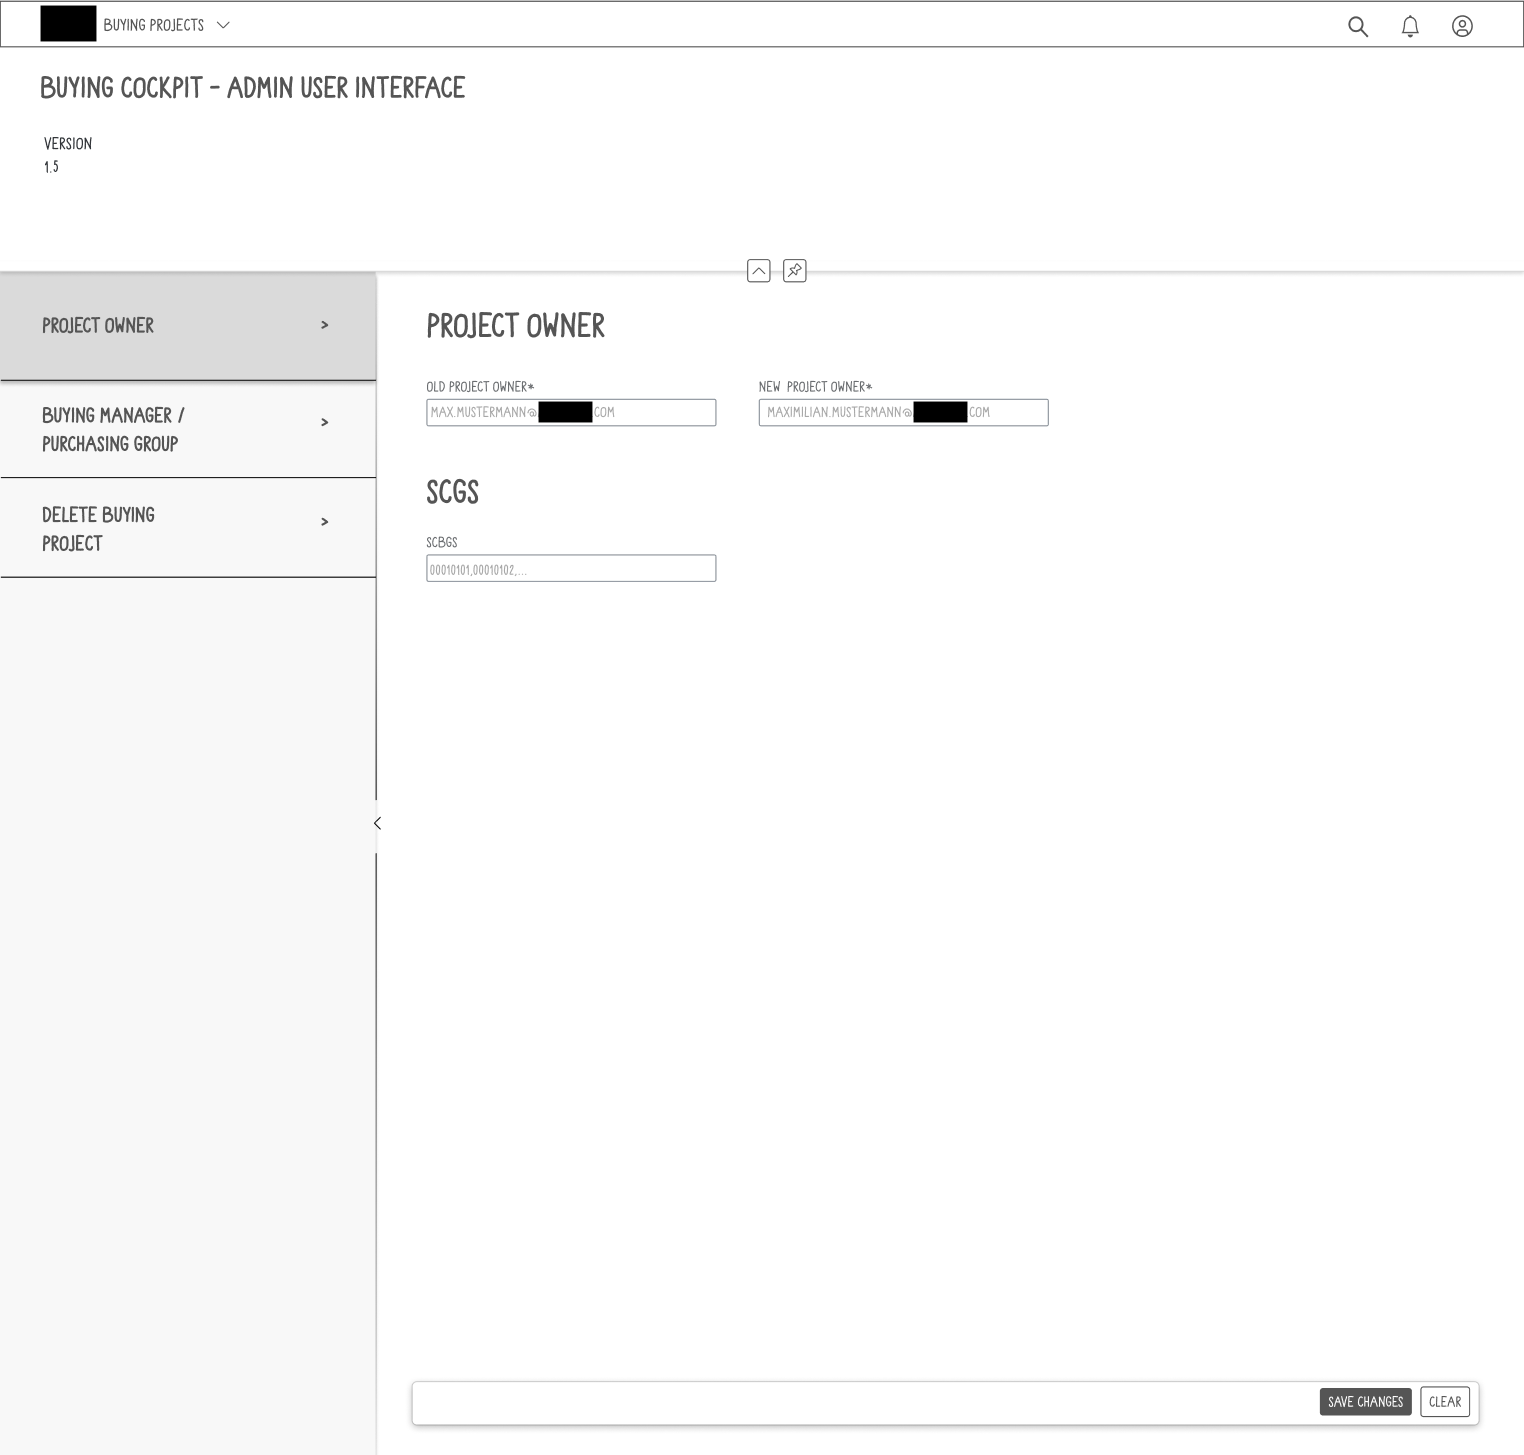
\includegraphics[width=\linewidth]{Images/Mockup_PO_anonym.png}
    \caption[Mockup: Admin-UI Projekowner Seite]{Mockup: Admin-UI Projekowner Seite}
\end{figure}

\begin{figure}[H]
    \centering
    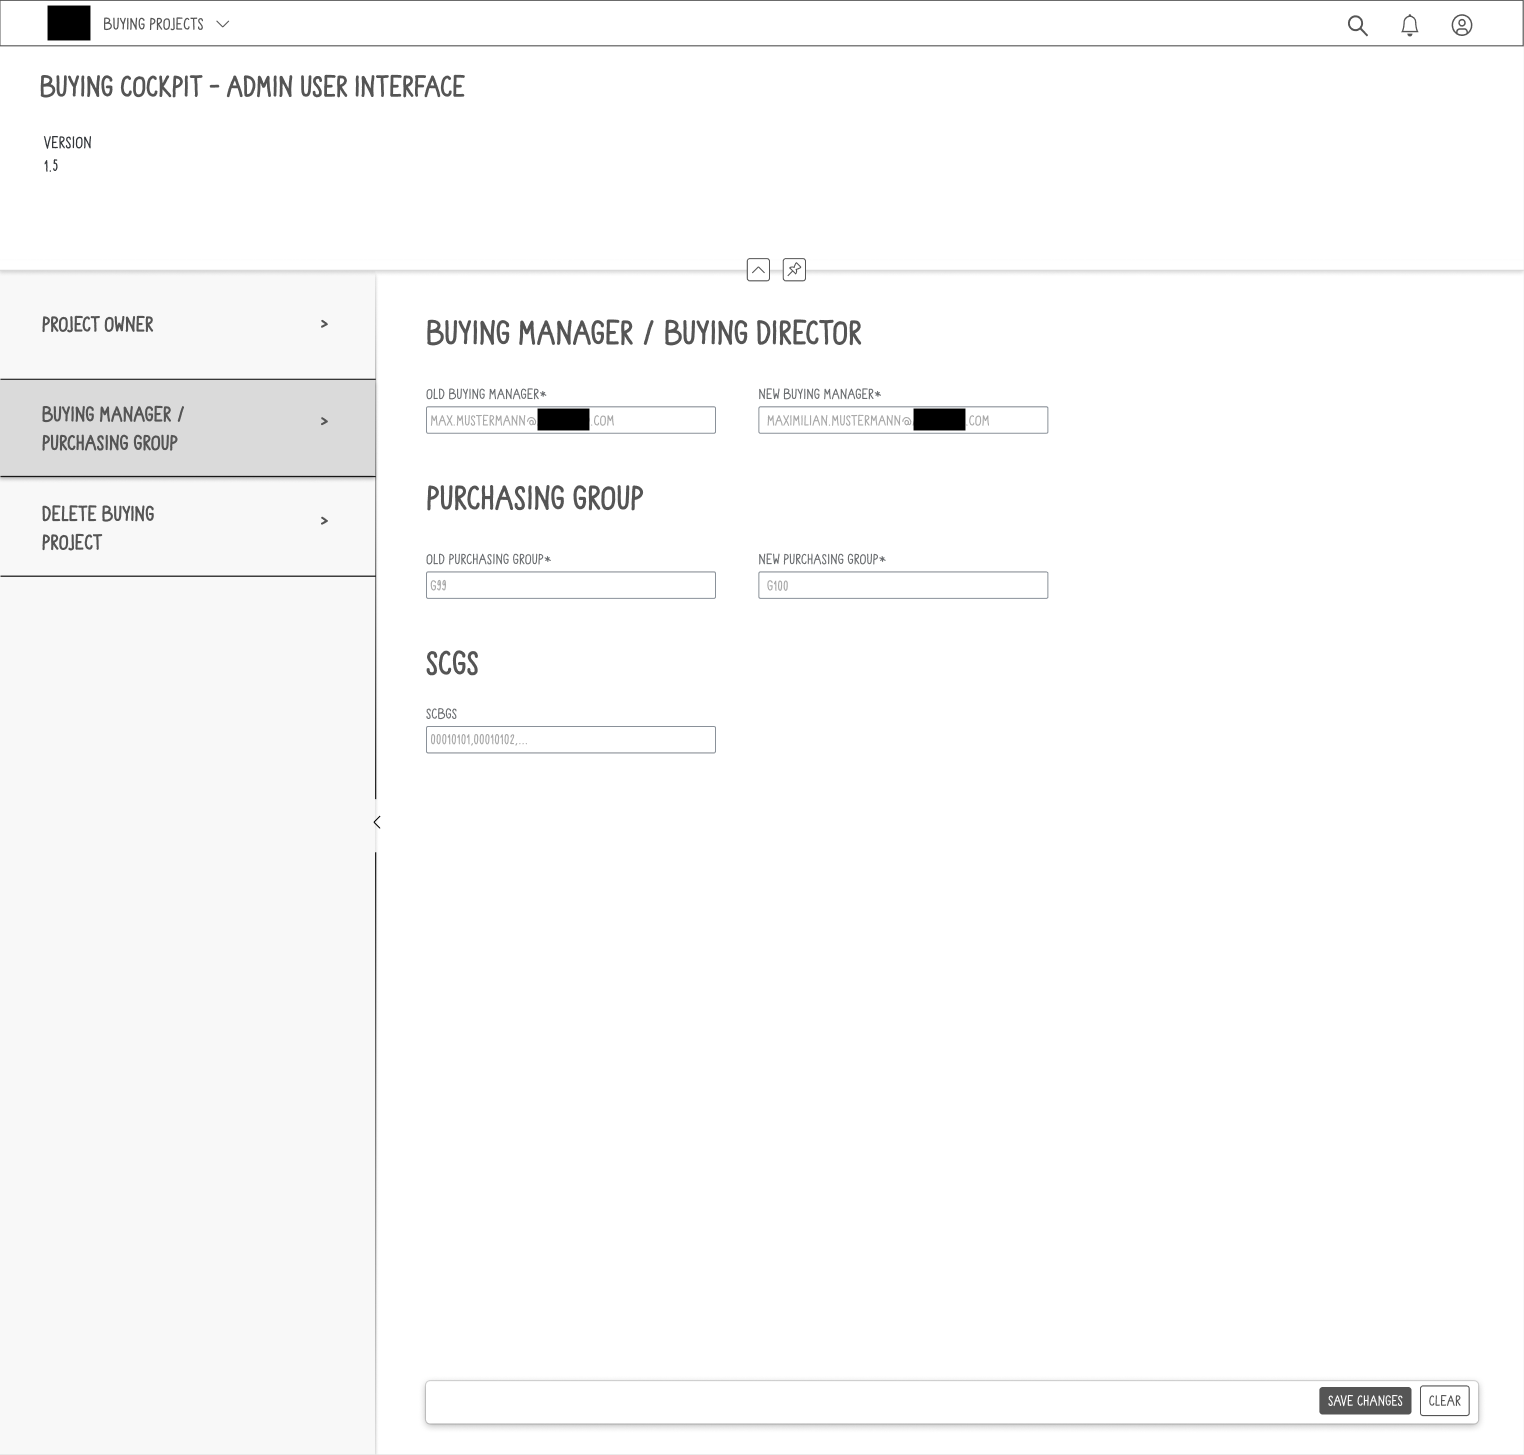
\includegraphics[width=\linewidth]{Images/Mockup_PM_anonym.png}
    \caption[Mockup: Admin-UI Projektmanager und Käufergruppe Seite]{Mockup: Admin-UI Projektmanager und Käufergruppe Seite}
\end{figure}

\begin{figure}[H]
    \centering
    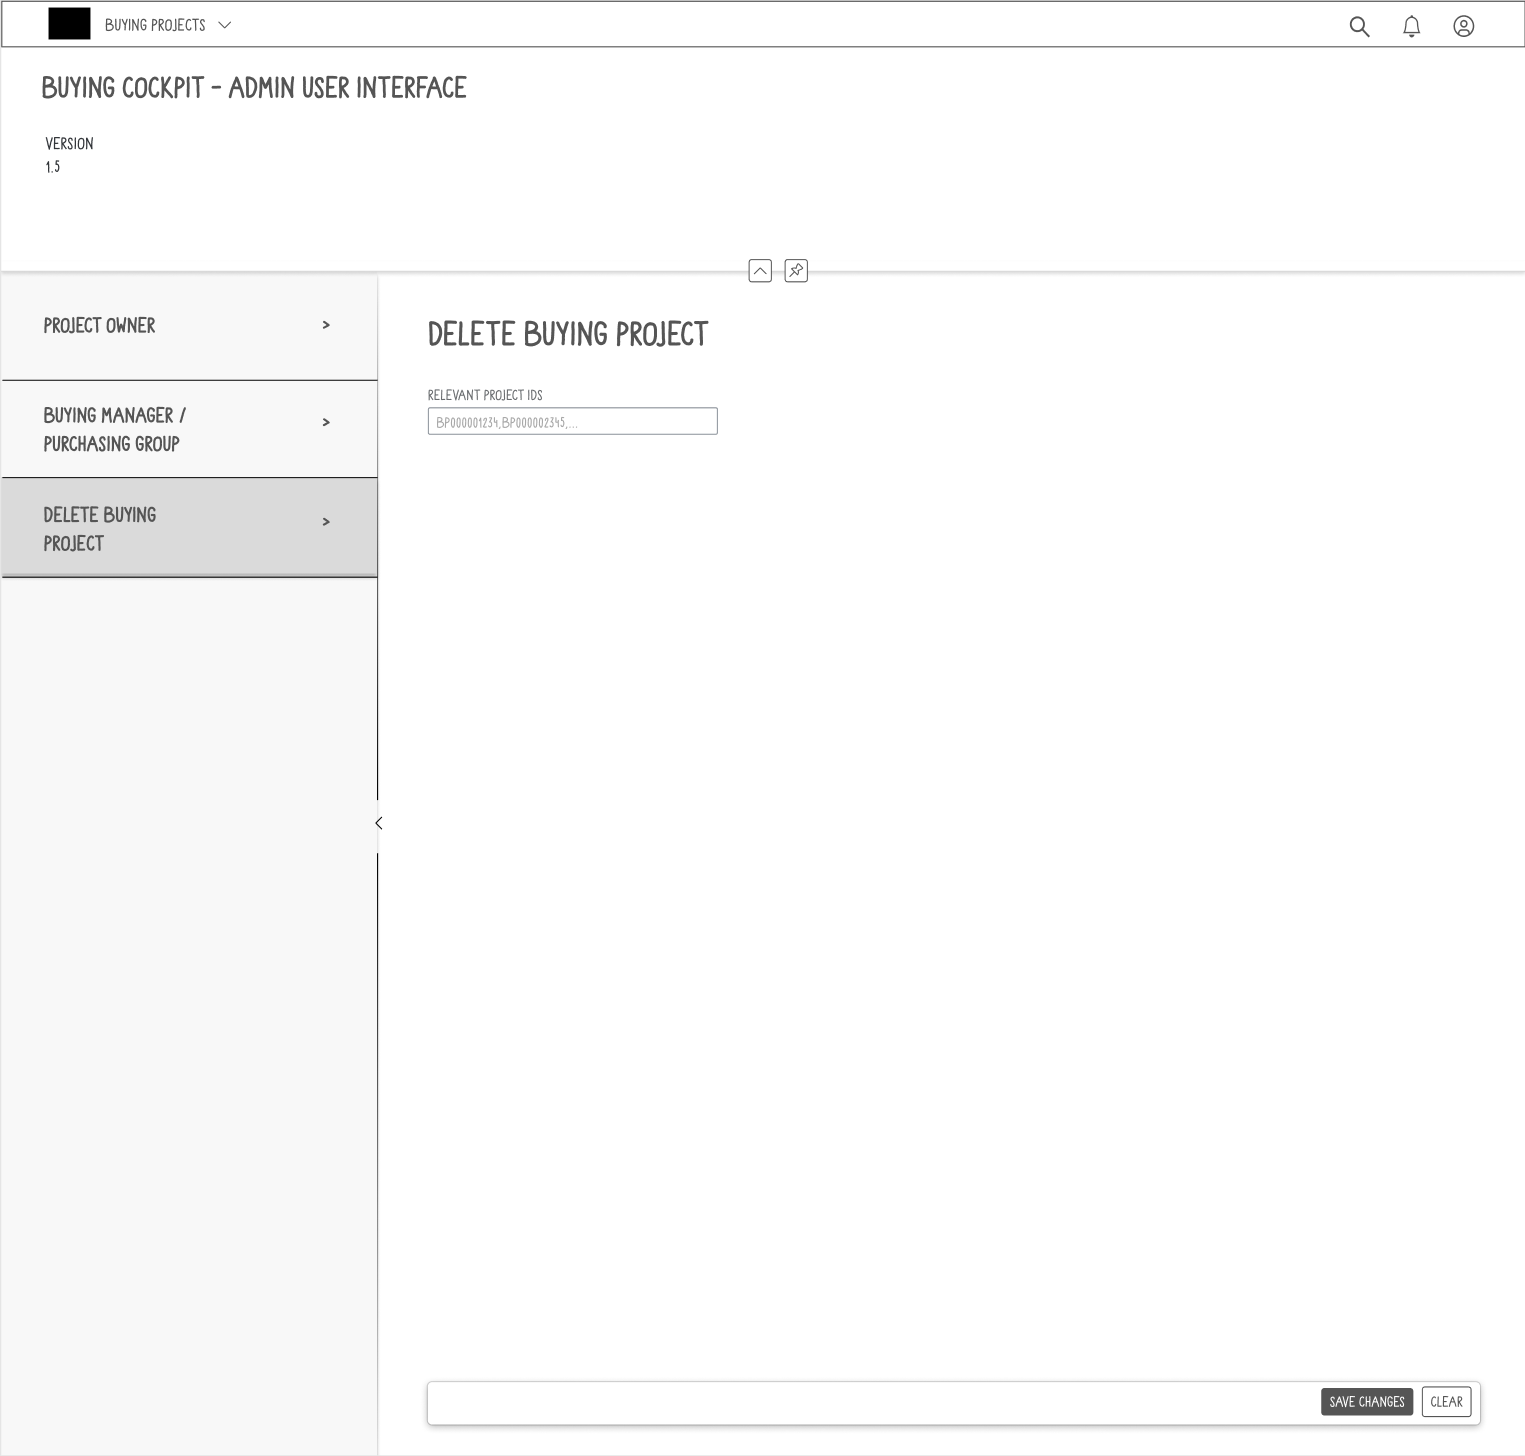
\includegraphics[width=\linewidth]{Images/Mockup_DEL_anonym.png}
    \caption[Mockup: Admin-UI Löschungs-Seite]{Mockup: Admin-UI Löschungs-Seite}
\end{figure}

\begin{figure}[H]
    \centering
    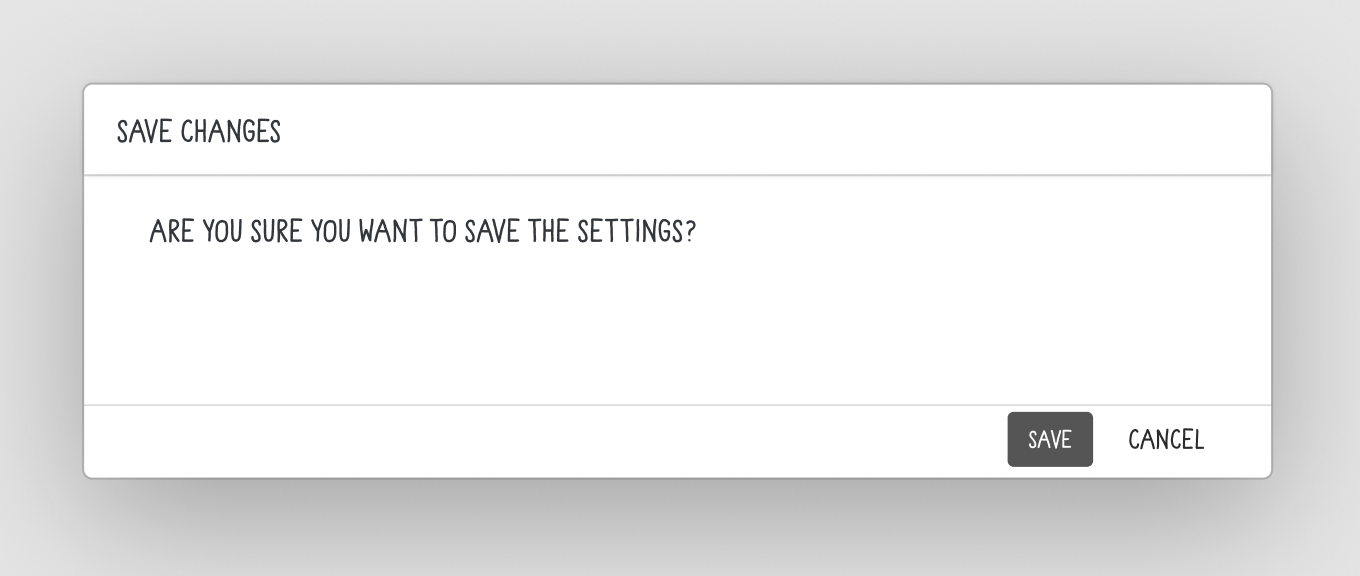
\includegraphics[width=\linewidth]{Images/Mockup_PopUp.png}
    \caption[Mockup: Admin-UI Pop-Up]{Mockup: Admin-UI Pop-Up}
\end{figure}

\subsection[Software-Design]{Software-Design}
Im folgenden Kapitel wird das Software-Design des Admin-UI und der dazu gehöhrenden Anwendung näher beschrieben.
Es bietet einen Überblick über die Architektur der Anwendung, die verwendeten Technologien und die Struktur der Daten.

\subsubsection[Grundlegende Architektur]{Grundlegende Architektur}
Die grundlegende Architektur der Anwendungen wird in Abbildung \ref{fig:architecture} etwas vereinfacht dargestellt, Komponenten, welche nicht relevant für die Entwicklung des Admin-UIs sind, wurden ausgelassen.

\begin{figure}[H]
    \centering
    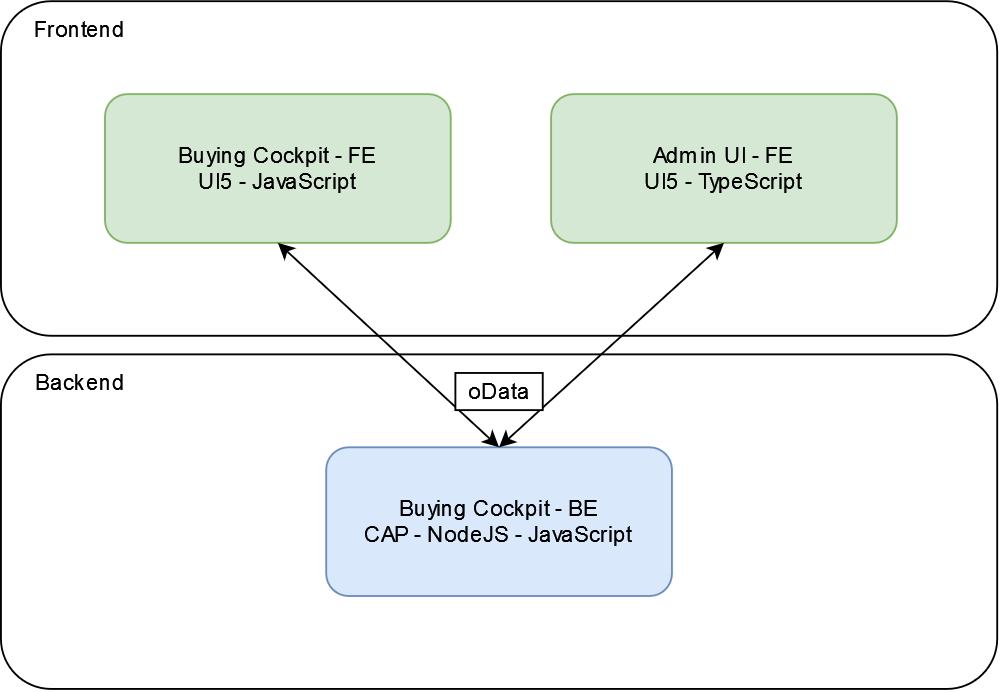
\includegraphics[width=\linewidth]{Images/BE_Architecture.png}
    \caption[Grundlegende Architektur der Anwendungen]{Grundlegende Architektur der Anwendungen}
    \label{fig:architecture}
\end{figure}
Die Architektur ist der Anwendungen ist in Frontend und Backend aufgeteilt und diese Ebenen kommunizieren über ein standartisiertes Protokol miteinander.

\begin{enumerate}
    \item \textbf{Frontend-Komponenten:}
    \begin{itemize}
        \item \textbf{Buying Cockpit - \gls{fe}:} \\
        Diese Komponente ist mit \gls{sapui5} und JavaScript entwickelt und bildet die Hauptanwendung und ist die Benutzeroberfläche für die Nutzer.
        \item \textbf{Admin-UI:} \\
        Dies ist die zu entwickelnde Administrationsoberfläche für das Buying Cockpit und  kann nur von bestimmten Nutzern verwendet werden.
    \end{itemize} 
    \item \textbf{Backend-Komponente:}
    \begin{itemize}
        \item \textbf{Buying Cockpit - \gls{be}:}
        Das Backend des Systems basiert auf \gls{cap} und wird mit NodeJS und JavaScript entwickelt.
        Es stellt die benötigten Daten und Services über standardisierte Schnittstellen beiden Frontend-Anwendungen zur Verfügung.
    \end{itemize}
    \item \textbf{Kommunikationsprotokoll:} \\
    Die Kommunikation zwischen dem Frontend und dem Backend erfolgt über das \textbf{OData-Protokol}. 
    \gls{odata} ermöglicht den standardisierten Austausch von Daten über HTTP und bietet eine effiziente Möglichkeit, auf Daten zuzugreifen und diese zu manipulieren.
\end{enumerate}
\subsubsection[Datenstruktur]{Datenstruktur}
Im folgenden wird die Datenstruktur für die Anwendungen vereinfacht dargestellt und Attribute, Entitäten und Relationen, welche nicht relevant für das Admin-UI sind, ausgelassen.

In Abbildung \ref{fig:datastructure} sind die drei Entitäten, welche im Admin-UI manipuliert werden sollen, in einen \gls{erm} dargestellt: \\
\begin{figure}[H]
    \centering
    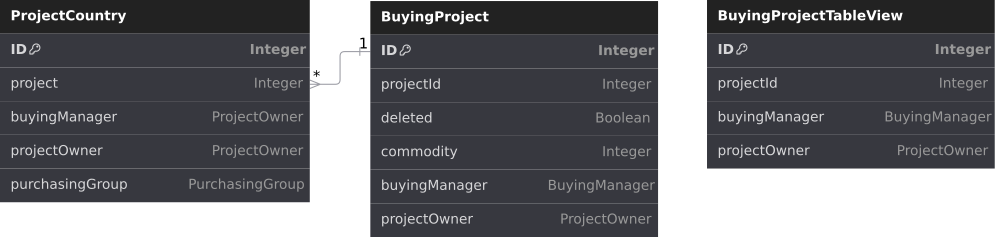
\includegraphics[width=\linewidth]{Images/Datenstruktur.png}
    \caption[Vereinfachte Darstellung der Datenstruktur]{Vereinfachte Darstellung der Datenstruktur}
    \label{fig:datastructure}
\end{figure}

Die Entität \textit{BuyingProjectTableView} ist eine Entität, welche für das Filtern auf der Übersichtsseite der BuyingCockpit Anwendung benötigt wird.
Daher müssen die Werte aus der \textit{BuyingProject}-Entität mit dieser übereinstimmen und somit immer beide simultan aktualisiert werden.
\section{Implementierung}
Dieses Kapitel beschreibt die Umsetzung des Projekts im Detail. Es wird ein Überblick über den Implementierungsprozesse gegeben, der Vorgehensweise bei der Entwicklung und ein Einblick in Probleme, welche während der Entwicklung aufgetreten sind.
Neben einer schrittweisen Darstellung der Implementierung werden auch exemplarisch Codebeispiele vorgestellt.
\subsection[Implementierungsdetails]{Implementierungsdetails}
In den Implementieungsdetails werden die Vorgehensweisen und Konzepte, welche für die Implementierung des Fontends und Backends benötigt werden, erläutert.

\subsubsection[Frontend]{Frontend}
Das \gls{sapui5}-Framework verwendet zur Darstellung der Seiten sogenannte \textit{Views} welche in \gls{xml} Dateien definiert werden.
Diese Views müssen mit der Dateiendung "\textbf{.view.xml}"\ enden, damit sie von \gls{sapui5} als View erkannt werden.

Views sind eine Art Kontainer für \gls{sapui5}-Elemente (Buttons, Input Felder, Tabellen, Listen, ...) und \gls{sapui5}-Layouts (Flex Box, HBox, VBox).
Views können jedoch auch andere Views beinhalten und so einen verschachtelten Aufbau der Seite schaffen.
Die \gls{sapui5}-Elemente sind vorgefertigte Komponenten welche von \gls{sapui5} bereitgestellt werden, um eine einheitliche Benutzeroberfläche zu schaffen, welche dann auch über verschiedene SAP-Anwendungen in einem Unternehmen konsistent ist.

Für die Admin-UI Seite sollen die Views und Komponenten wie in Abbildung \ref{fig:appstructure} angeortnent und strukturiert werden.
Die Unterseiten für die Eingabefelder aus den Anforderungen \ref{Tab:A4}, \ref{Tab:A5} und \ref{Tab:A6} werden in eigenen Views angezeigt, zwischen denen der Benutzer über die Navigationsleiste wechseln kann.

\begin{figure}[H]
    \centering
    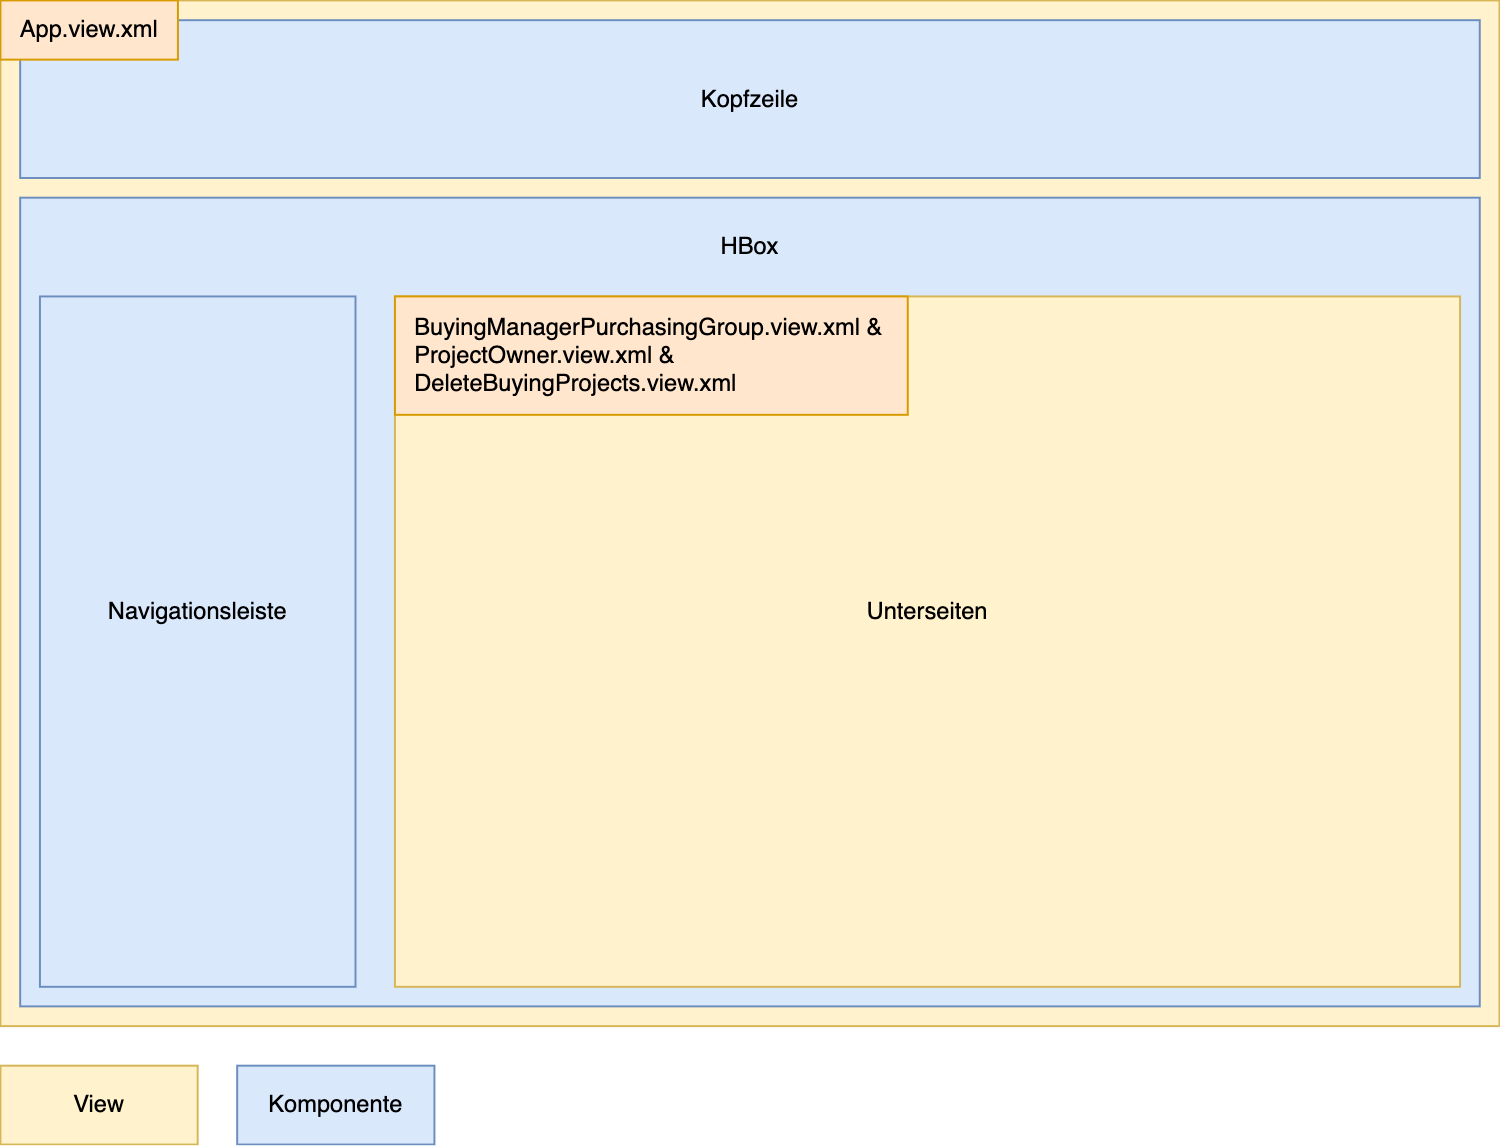
\includegraphics[width=\linewidth]{Images/AppStructure.png}
    \caption[Darstellung der Anwendungsstruktur]{Darstellung der Anwendungsstruktur}
    \label{fig:appstructure}
\end{figure}

Für jeden View kann ein \textit{Controller} erstellt werden, welcher die Funktionalität für die Views bereitstellt und Elemente dynamisch laden kann. 
Ein muss, so wie die View, eine besondere Dateiendung haben, damit \gls{sapui5} die Datei als Controller erkennen kann. Für Controller ist diese Endung "\textbf{.controller.ts}".

Für das Admin-UI soll für jeden View ein Controller erstellt werden. Zudem soll es einen sogenannten \textit{BaseContoller} geben, von dem alle anderen Controller seine Funktionen erben.
Dieser BaseController benötigt, anders also normale Controller, nicht die Controller spezifische Endung sondern nur die TypeScript spezifische Dateiendung "\textbf{.ts}".
Denn der BaseController wird keinem View explizit zugeordnet und muss daher auch nicht von \gls{sapui5} als Controller erkannt werden.  

Die Funktion eines BaseControllers ist es, Funktionen, welche von jedem Controller benötigt werden, in diesem zu definieren, damit diese an einer zentralen Stelle definiert sind und nicht in jedem Controller neu defniert werden müssen. 
Dazu gehören meist Helferfunktionen für zum Beispiel das Routing oder im Fall des Admin-UIs auch die Funktionalität der Aktionsleiste (siehe Anforderung \ref{Tab:A7}), welche auf jeder Unterseite eine sehr ähnliche Funktion hat.

In den Controllern für die einzelnen Unterseiten sollen Funktionen die spezifisch für die Unterseiten sind stehen, wie die intelligenten Vorschläge für die Eingabefelder (Anforderung \ref{Tab:A3}) und das Senden der Daten an das Backend.

\subsubsection[Backend]{Backend}
Im Backend sollen die Daten, welche von dem Frontend gesendet wurden, validiert und verarbeitet werden.

Für das Löschen einen Kaufprojekts muss jediglich die \textit{projectId} des zu löschenden Projektes gesendet werden, wofür eine \gls{cap} \textit{function} verwendet werden soll.
Eine \gls{cap} \textit{function} kann Parameter haben und muss immer einen Rückgabewert haben und führt eine gewisse Aktion aus.

Für das Ändern der Projekt Owner und Manager, sowie der Purchasing Organisation, soll für jede Änderung ein neuer Eintag in eine Datenbanktabelle geschrieben werden, der die alten und neuen Werte, sowie den Benutzer der die Änderung getätigt hat und den Zeitpunkt der Änderung beinhaltet.
Diese Datenbanktabellen sind in Abbildung \ref{fig:masschangetables} dargestellt.
Dies soll dazu dienen, die Änderungen auch im Nachhinein nachvollziehen zu können oder auch Rückgeängig zu machen. 

\begin{figure}[H]
    \centering
    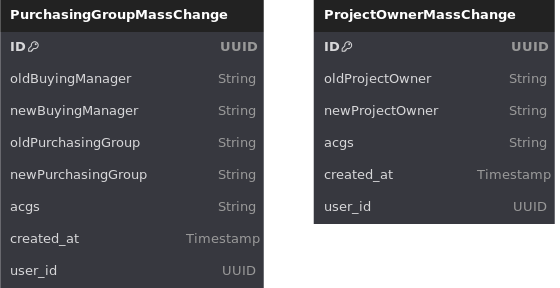
\includegraphics[width=.6\linewidth]{Images/MassChangeTables.png}
    \caption[Datenbanktabellen für Massenänderungen]{Datenbanktabellen für Massenänderungen}
    \label{fig:masschangetables}
\end{figure}

Wenn aus dem Frontend ein neuer Eintrag in einer der Tabelle erstellt wird, soll mit einer sogenannten \textit{Hook} in \gls{cap} das Änderen der Daten geschehen.
Diese \textit{Hooks} fangen das Erstellen der Tabelle ab und führen dann individuellen Code aus, in dem die gesendeten Daten verarbeitet werden können.

Bevor jedoch die Daten verarbeitet werden, muss überprüft werden, ob der Benutzer, der die Daten gesendet hat, die Berechtigung hat diese Änderungen durchzuführen.
Falls dies nicht der Fall ist, soll ein Error an das Frontend gesendet werden und eine entsprechende Errornachricht angezeigt werden.
Wenn der Benutzer jedoch die benötigte Berechtigung besitzt sollen die Daten verarbeitet und validiert werden und die Änderungen in der Datenbank vorgenommen werden.

\subsection[Schrittweise Beschreibung der Implementierung]{Schrittweise Beschreibung der Implementierung}

In diesem Abschnitt werden die Implementierungsdetails aus dem vorherigen Abschnitt anhand von Codebeispielen schrittweise erläutert und erklärt.

\subsubsection{Frontend}
Die Implementierung des Frontends teilt sich in zwei Abschnitte auf. 
Zum einen die Erstellung der Views, welche die Darstellung der Seite seien werden, und die Erstellung der Controller, zum anderen die Views mit Funktionalität zu versehen. 

\textbf{Erstellung der XML-Views:}

Für die Darstellung wurden, wie in Abbildung \ref{fig:appstructure} bereits dargestellt wurde, vier verschiende \gls{xml}-Views angelegt.
Die \textit{App.view.xml}, \textit{BuyingManagerPurchasingGroup.view.xml}, \textit{ProjectOwner.view.xml} und die \textit{DeleteBuyingProjects.view.xml}.

Für die App-View wurden drei Hauptkomponenten benötigt.
Die Kopfzeile mit dem Titel der Seite, die Navigationsleiste zur Navigation zwischen den Unterseiten und die Unterseiten an sich, welche dynamisch mit Hilfe der Naviagtionsleiste angezeigt werden.
All diese Komponenten wurden innerhalb einer \textit{DynamicPage-Komponente} definiert, welche bereits Funktionalitäten für eine einfahrbare Kopfzeile und Navigationsleiste bietet.
So konnte die Kopfzeile als eine \textit{DynamicPageTitle und DynamicPageHeader-Komponente} als Titel und Header der DynamicPage hinzugefügt werden.
Wie das dann im Code für das Admin-UI aussieht, sehen Sie im folgenden Listing:

\begin{lstlisting}[caption={Kopfzeile des App-Views}, language={XML}]
<f:DynamicPage class="sapUiNoContentPadding">
    <f:title>
        <f:DynamicPageTitle>
            <f:heading>
                <Title text="{i18n>titHeader}" class="sapUiSmallMarginTop" />
            </f:heading>
        </f:DynamicPageTitle>
    </f:title>
    <f:header>
        <f:DynamicPageHeader>
            <VBox>
                <Label text="{i18n>lblVersion}" />
            </VBox>
        </f:DynamicPageHeader>
    </f:header>
    ...
</f:DynamicPage>
\end{lstlisting}

Das \textit{text}-Attribut, liefert den Text der in dem Titel und dem Header angezeigt werden.
Dieser kommt in unserem Fall aus dem \textit{i18n}-Model, welches Text in verschiedenen Sprachen bereitstellt.
Das \textit{class}-Attribut, ist für das Styling der Elemente verantwortlich. 
Hier wird eine von \gls{sapui5} vorgefertige Klasse angegeben, um ein einheitliches Aussehen auf der ganzen Seite zu garantieren.

Für die Navigationsleite und die Unterseiten wurden zwei \textit{Panel-Komponenten} verwendet, diese dienen als Kontainer für den Inhalt der Komponenten und haben die Möglichkeit sich ein- und ausklappen zu lassen.
Die Navigationsleite wurde als eine Liste von \textit{ActionListItems} definiert, welche eine Art Knöpfe sind, die durch Attribute als ausgewählt angezeigt werden können.
Diese \textit{ActionListItems} werden anhand von vordefinerten Routen dynamisch generiert und sind somit jeweils an eine Route, beziehungsweise an eine Unterseite gebunden.
Durch anklicken eines der \textit{ActionListItems} wird über den \gls{sapui5}-Router das richtige XML-View in den \textit{Panel-Kontainer} für die Unterseiten geladen.

In dem folgenden Listing wird der Code für die beiden \textit{Panel-Komponenten} dargestellt, es wurden jedoch Attribute und Elemente, welche jediglich für das Aussehen der Komonenten zuständig sich, ausgelassen. 

\begin{lstlisting}[caption={Navigationsleisten- und Unterseiten-Kontainer des Admin-UIs}, language={XML}]
...
<Panel>
    <List items="{routes>/routes}">
        <ActionListItem
            text="{
                parts: [
                    'routes>name'
                ], formatter: '.formatter.formatNavItemText'
            }"
            type="Navigation"
            navigated="{= ${routes>name} === ${routes>/currentRoute}}"
            press="onNavItemPress" />
    </List>
</Panel>
<Panel>
    <NavContainer id="navContainer" width="100%" height="100%" />
</Panel>
...
\end{lstlisting}

Die drei \gls{xml}-Views für die Unterseiten sind alle gleich aufgebaut und verwenden alle dieselben Komonenten zur Darstellung der \textit{Toolbar} zum Speichern der Änderungen und den Eingabefeldern.

Für die Toolbar wird die \textit{Toolbar-Komponente} von \gls{sapui5} verwendet und beinhaltet zwei Knöpfe.
Ein Knopf zum Speichern und ein Knopf, um alle Eingabefelder zu leeren. 
Im folgenden Listing wird der Code für die Toolbar, welche auf allen Seiten weitestgehend identisch ist, dargestellt:

\begin{lstlisting}[caption={Toolbar der Unterseiten}, label={lst:toolbar}, language={XML}]
<Toolbar id="toolbar" design="Solid">
    <ToolbarSpacer />
    <Button text="{i18n>btnSaveChanges}" type="Emphasized" press="onSaveChangesPress" />
    <Button text="{i18n>btnClear}" press="onClearPress" />
</Toolbar>
\end{lstlisting}

Die Eingabefelder wurden mit \textit{Input-Komponenten} umgesetzt, da diese bereits Funktionalitäten für intelligente Vorschläge, wie in Anforderung \ref{Tab:A3} beschreiben, besitzen.
Für eine bessere Formatierung wurde jedes Eingabefeld und dessen Titel, welcher als \textit{Label-Komponente} dargestellt wird, in einer \textit{VBox-Komponente} platziert.
In dem folgenden Listing wird der Code für das Eingabefeld beispielshaft an einem Eingabefeld auf der ProjectOwner.view.xml Unterseite dargestellt:

\begin{lstlisting}[caption={Eingabefeld für Unterseiten}, language={XML}]
<VBox width="100%">
    <Label text="{i18n>lblOldBuyingManager}" required="true" />
    <Input
        id="oldBuyingManagerInput"
        value="{form>/oldBuyingManager}"
        placeholder="{i18n>txtEmailPlaceholder1}"
        required="true"
        suggestionItems="{/AppUsers}"
        showSuggestion="true"
        suggest="onSuggest($event, 'user')"
        suggestionItemSelected="onSuggestionItemSelected">
        <core:Item key="{id}" text="{id}" />
    </Input>
</VBox>
\end{lstlisting}

Die Attribute \textit{suggest} und \textit{suggestionItemSelected} der Input-Komponente bekommen die Namen von Funktionen übergeben, welche in einem Controller für die Views definiert sind.
Die Funktion dieser Funktionen ist es die intelligenten Vorschläge anhand der Benutzereingabe anzuzeigen und beim Auswählen eines der Vorschläge diesen Wert für das Feld zu übernehmen.
Das Attribut \textit{required} ist dafür da anzuzeigen, ob das Eingabefeld ein Pflichfeld ist und es dieses auf \textit{true} gesetzt wird vor dem Speichern überprüft, ob in diesem Feld etwas eingegeben wurde.

\textbf{Erstellung der Controller:}

Eingie Funktionalitäten sind in allen Unterseiten identisch, daher wurde für diese Funktionen ein BaseController erstellt.
Funktionen in diesem Contoller, stehen allen Views zur Verfügung, wodurch der Code für diese Funktionalitäten nur ein mal geschreiben werden musste.

Andere Funktionalitäten sind jedoch spezifisch für eine Unterseite oder muss unterschiedlich implementiert werden, da es zum Beispielt unterschiedlich Eingabefelder auf den Seiten gibt.
Eine dieser Funktionen ist die \textit{onSaveChangesPress}-Funktion aus Listing \ref{lst:toolbar}, die für das Speichern der Eingabefelder zuständig ist.

\begin{lstlisting}[caption={onSaveChangesPress Funktion}]
onSaveChangesPress(event: Button$PressEvent): void {
    const formModel = this.getModel<JSONModel>("form"),
            isFormValid = this.validateInputFields(this.allInputIDs);

    if (!isFormValid) {
        event.getSource().setEnabled(false);
        return;
    }

    if (!formModel) return;

    const {
        oldProjectOwner,
        newProjectOwner,
        SCGs
    } = formModel.getData();

    this.createSaveChangesMessageBox(
        "/ProjectOwnerMassChange", 
        {                
            oldProjectOwner,
            newProjectOwner,
            acgs: SCGs
        },
        this.allInputIDs
    );
}
\end{lstlisting}

In dieser Funktion werdern die Eingabefeld validiert, indem überprüft wird, ob all Pflichtfelder ausgefüllt sind.
Wenn dies der Fall ist, wird mit den Werten der Eingabefelder ein neuer Tabelleneintrag im Backend erstellt.
Der Tabellenname ist für die verschiedenen Unterseiten unterschiedlich und daher wird dieser zusammen mit den Daten an die \textit{createSaveChangesMessageBox}-Funktion im BaseController gesendet.
Diese Funktion ist im folgenden Listing zu sehen:

\begin{lstlisting}[caption={createSaveChangesMessageBox Funktion}]
protected createSaveChangesMessageBox(sPath: string, formData: object, inputIDs: string[]): void {
    const resourceBundle = this.getI18nResourceBundle();
    if (!resourceBundle) {
        return;
    }

    const saveAction = resourceBundle.getText("btnSave") || "Save";
    MessageBox.confirm(
        resourceBundle.getText("txtConfirmDialog") || "",
        {
            title: resourceBundle.getText("titConfirmDialog") || "",
            actions: [saveAction, MessageBox.Action.CANCEL],
            emphasizedAction: saveAction,
            onClose: (action: string) => {
                if (action === saveAction) {
                    this.submitChanges(sPath, formData, inputIDs);
                }
            }
        }
    );
} 
\end{lstlisting}

Dies ist eine Funktion im BaseController, welche eine \textit{MessageBox-Komponente} erstellt, um den Nutzer um eine weitere Bestätigung zu bitten.
Bestätigt der Benutzer seine Entscheidung, wird die \textit{submitChanges}-Funktion aufgerufen.

\begin{lstlisting}[caption={submitChanges Funktion}]
protected submitChanges(sPath: string, oData: object, inputIDs: string[]): void {
    const   viewModel = this.getModel<JSONModel>("objectView"),
            model = this.getModel<ODataModel>();

    if (!model || !viewModel) return;

    viewModel.setProperty("/busy", true);
    model.create(sPath, oData,
        {
            success: () => {
                this.clearAllFields(inputIDs);
                this.onSubmitSuccess();
            },
            error: this.onSubmitError.bind(this),
        }
    );
} 
\end{lstlisting}

Diese Funktion ist dafür verantwortlich die übergebenen Daten an das Backend zu senden.
Um das zu tun wird in dem \gls{odata}-Model, welches mit dem Backend verbunden ist, ein neuer Eintrag erstellt.
Dafür benötigt es die Namen der Tabelle, sowie die Daten, die in die Tabelle geschrieben werden sollen.
Ist das Erstellen des neuen Eintrages erfolgreich, werden alle Eingabefelder geleert und es wird eine Meldung angezeigt, dass das Speichern erfolgreich war.
Im Fall, dass das Erstellen nicht erfolgreich war wird eine Errornachricht angezeigt.

\subsubsection[Backend]{Backend}

Nachdem die Daten von dem Frontend an das Backend gesendet wurden müssen diese Dort noch verarbeitet werden und die von den Änderungen betroffenen Tabellen müssen bearbeitet werden.
Die Beschreibung dieser Funktionalität wird im folgenden schrittweise beschrieben.

Sobald im Frontend eine Anfrage an das Backend gesendet wird, um einen neuen Eintrag in der Tabelle zu erstellen, wird diese Anfrage von SAP CAP abgefangen. Dies geschieht in der srv.on Funktion, welche bestimmte Events abfangen kann. Sie hat drei Parameter, das Event, welches abgefangen werden soll, den Namen der Entität und eine Handlerfunktion, die aufgeführt wird, wenn eine Anfrage abgefangen wurde.

In diesem Fall ist das Event das “CREATE” Event, welches beim Erstellen eines neuen Eintrags aufgerufen wird. Der Name der Entität ist abhängig von der Unterseite von der die Anfrage gestellt wurde. Die Handlerfunktion hat zwei Parameter, die Anfrage, in der die Daten die gesendet wurden sowie weitere Informationen über die Anfrage, wie den Benutzer, der die Anfrage gestellt hat, stehen.

Im folgenden wird das Codebeispiel nur für eine der Funktionalitäten dargestellt, da der einzige Unterschied die aufgerufene Funktion, ist.
```
srv.on('CREATE', 'PurchasingGroupMassChange', async (req, next) => {
        const whitelistedMassChangeUsers = process.env.ADMIN_UI_USERS ? process.env.ADMIN_UI_USERS.split(',') : []
        if(whitelistedMassChangeUsers.indexOf(req.user.id.toLowerCase()) < 0) {
            req.error(400, 'Invalid user')
        } else {
            try {
                await projectService.purchasingGroupMassChange(req)
                return await next()
            } catch (e) {
                logAndThrowError(log, 'performing purchasing group mass change', e, req.data)
            }
        }
    })
```
Caption: srv.on Funktion zum Abfangen der Anfrage

In unserer Handlerfunktion ist das erste was geprüft wird, ob der Benutzer der die Anfrage gestellt hat, die passenden Rechte für eine solche Anfrage besitzt. Ist dies nicht der Fall, wird eine Errornachricht zurück gesendet. Besitzt der Benutzer die passenden Rechte, wird eine Funktion aufgerufen, welche die Validierung und Verarbeitung der Daten übernimmt.

In dieser Funktion werden zuerst die Daten Validiert. Dafür wird überprüft, ob alle benötigten Daten angekommen sind und ob diese das korrekte Format besitzen. Falls dies nicht der Fall ist, wird eine Errornachricht zurück gesendet. Nachdem die Validierung abgeschlossen ist und es zu keinem Error kam, werden die betroffenen Entitäten aktualisiert. 




\subsection[Herausforderungen und Problemlösungen]{Herausforderungen und Problemlösungen}

\subsection[Beschreibung der Lösungsansätze]{Beschreibung der Lösungsansätze}

\section{Fazit}

\subsection[Zusammenfassung der Arbeit]{Zusammenfassung der Arbeit}

\pagestyle{plain}

% References
\newpage
\addcontentsline{toc}{chapter}{Bibliography}
\printbibliography

% Figures
\newpage
\addcontentsline{toc}{chapter}{Abbildungsverzeichnis}
\listoffigures
% Tables
\newpage
\addcontentsline{toc}{chapter}{Tabellenverzeichnis}
\listoftables
% Listings
\newpage
\addcontentsline{toc}{chapter}{Quellcodeverzeichnis}
\lstlistoflistings
\newpage
% ============================================

\chapter*{Abkürzungsverzeichnis}
\begin{acronym}
    \acro{scg}[SCG]{Sales Category Group} 
    \acroplural{scg}[SCGs]{Sales Category Groups}
\end{acronym}
Eine \ac{scg} ist ein kundeninterne Nummer die Produktgruppen kategoriesiert. 

\begin{acronym}
    \acro{sapui5}[SAPUI5]{SAP User Interface 5}
\end{acronym}
\acs{sapui5} ist ein Frontend Framework von SAP.

\begin{acronym}
    \acro{cap}[SAP CAP]{SAP Cloud Application Programming Model}
\end{acronym}
\acs{cap} ist ein Backend Framework von SAP.

\begin{acronym}
    \acro{ide}[IDE]{Integrated Development Environment}
    \acroplural{ide}[IDEs]{Integrated Development Environment}
\end{acronym}
Eine \ac{ide} ist eine Softwareanwendung, welche Entwicklern beim Schreiben von Programmen unterstützen soll.

\begin{acronym}
    \acro{oop}[OOP]{Objektorientierte Programmierung}
\end{acronym}
\ac{oop} ist ein Modell der Computerprogrammierung, bei dem das Softwaredesign auf Daten oder Objekten basiert und nicht auf Funktionen und Logik.

\begin{acronym} 
    \acro{sql}[SQL]{Structured Query Language}
\end{acronym}
\acs{sql} ist eine Datenbanksprache zur Definition von Datenstrukturen in relationalen Datenbanken
\chapter[Quellen]{Quellen} 
\begin{itemize}
    \item https://ui5.sap.com/
    \item https://sap.github.io/ui5-typescript/
    \item 
\end{itemize}



% ============================================

\end{document}

